\chapter{Agent-based modelling \label{chapter:ABM}}

\begin{comment}
BITS FOR THIS CHAPTER
%===============================

WUD 24	Very different market structures possible for agents. Cf. actor-centric vs actor-firm. Difference in outcome?
MM2 76	Different way to approach two goods. Cf. other model choices.
-- Backyard-style collaboration at SoCs each making one good (because of EoS). 
-- Actors get their share, and can then trade, Edgeworth-style, to get a better bundle.

%cf. prod functions
FDA 5	Cognition and black boxes: utility / psychology, production/UNSW coffee stand/Jacobs. 1940 committee to sort out utility.
WUD 14	When are black boxes OK? More on WUD 26.

%In econs, intro to basic use of equilibrium. Key problem: assumptions of e.g. zero profit; massively useful for analytics, not important for ABM and possibly get in the way. Cf. Brakman on Fowler.
WUD 3	Equilibrium: strong and weak arguments. E.g. as both Krugman and Isard argue, though Krugman not in any depth: we don't believe they exist in the real world, only that the real world tries to reach them. It never succeeds, but in understanding the equilibria, we can understand the processes of change that are going on in the real economy.

WUD 4	Equilibrium in Fowler and Brakman. Go back to.
WUD 6	Fowler2 points out `equilibrium assumed a priori'. Cf. objects at rest.

WUD 20	Straight to PhD: section on agent numbers. They're there to get effect of heterogenous interaction, not to exactly match real-world numbers.

WUD 27	Zotero 'Jacobs' search - lots!
WUD 24	Agent-based models are all knowledge economy. Cf Jacobs again!
MM2 43	A finite amount of capital has to do the work of sending the appropriate signals.
MM2 68	Data, meaning, appropriate response table. Might be useful.

MM1 41	What are the different limitations that money supply, stock levels, prices place on the model? I've tried giving them heaps more money; it's quite a different dynamic�

MM2 65	The crash problem: firms underbid each other, stock eventually so cheap that it's all bought out. Model locks.
MM2 65	Discussion: the more blindly agents can find optima, the more one can say the objectively exist?

MM2 71	Money supply problem, plus money as a factor: if wage demands exceed money supply, some work won't get done and some goods won't get bought. In a situation where people are randomly looking for work, some will succeed, others not - randomly - as wage payments exceed available capital. In a situation where there are economies of scale to be had, if our one firm is missing out on labour input because of a lack of money supply, the economy as a whole is missing out on welfare gains.
There's also a relationship between prices and velocity: goods cost might be high and wages high also; money will pass through the one firm faster than if those are both lower. (Need to read some Friedman!)
But might it also be possible for the following to happen: if the price is lowered on the good, quantity goes up in a non-revenue increasing way? Well, of course it is: that would be an inelastic PED: decreasing price may increase quantity bought, but decreases total revenue. And if there's only one firm, decreasing total revenue knocks on to decreasing ability to pay wages... 
So the question is: do stock levels - does the productivity from economies of scale - necessarily have to have anything to do with where prices are set? Is it actually a reasonable economic outcome for constantly increasing stock to result? And, how do we find out?
(The above text is taken from a lyx document in dropbox/java/twogoods1/notes.)


\end{comment}
%===============================

%Intro quote
\vspace{2cm}
%http://www.youtube.com/watch?v=wMFPe-DwULM
\begin{quote}
{\large
``When you explain a `why', you have to be in some framework that you allow something to be true. Otherwise you are perpetually asking why.''
\\
\hspace*{10cm}\emph{Richard Feynman\footnote{In interview on `Fun to Imagine,' BBC, 1983.}}}
}
\end{quote}

\vspace{2cm}

%\section{Introduction to chapter \label{ABMintro}}

%conceptual apparatus! Di Paulo. 

\section{What is agent-based modelling?}

\gls{abm}, as the name suggests, simulates `agents': distinct code objects, programmed to interact with their environment and each other. \gls{abm} developed in tandem with \gls{oop}. Though \gls{oop} has a history going back to the sixties, it was not until the nineties that computing power and programming languages like Java developed enough to mark a `paradigm shift' in programming (\citealt{robinson_emergence_2009} p.211). This shift provided the soil for \gls{abm} to flourish. 

%The objects in \gls{oop} differ from more standard functions in their multi-faceted structure. 
Wooldridge defines objects as ``computational entities that \emp{encapsulate} some state, are able to perform actions, or \emph{methods}, on this state, and communicate by message passing'' (\citealt{wooldridge_introduction_2009} p.28). Objects are created from classes; a real-world metaphor would be that classes are the blueprint and objects the physical form. Thus, a model may have a single `Firm' class but many `Firms' created from that blueprint, with their own internal state.

This focus on objects' `encapsulation' - that `objects have control over their own internal state' - requires the programmer to think of them as separate entities, and to define inter-relations with care. (The procedural element of programming has not gone away, however, and is still of vital importance, particularly with regard to timings; see section \ref{sec:actions}.) A popular online java tutorial (\citealt{the_java_tutorials_what_????}) has a simple illustration of encapsulation: if a rider of a bicycle attempts to change gear, the bicycle should have a `method' that ensures it cannot exceed its gear number. The rider is denied the ability to \emph{force} a gear-change above those available. In coding practice, this mean providing methods to raise and lower gears: the rider may \emp{`request'} a gear change, but the bicycle `decides' if it can be done.

This trivially simple idea, in conjunction with a set of supporting \gls{oop} coding concepts, has created a very powerful set of tools for defining how objects interact. 
%`a preditable effect...' woz ere.

\subsection{Mapping: code versus function \label{sec:mapping}}

Some cuttings:

influence of MONIAC on Keynesians - \citealt{wood_john_1994} p.249, which notes even over this, there were arguments about the `misleading reduction of economics to hydraulics' (\citealt{shackle_years_1983} p.189 in \citealt{wood_john_1994} p.249)

ironic, given that Newyln himself was well aware of this limitation: ``once the model has served its purpose... the student will need to return to the literature for the complications and refinements - hydraulics is no substitute for economics.'' (\citealt{newlyn_phillips/newlyn_1950} p.119)

Point I want to make there again, it is the job of the modeller to define the purpose of the model; it is incumbent on others who want to comment to try and understand what the modeller wanted to achieve; it is also entirely possible for models to develop a form of `mission creep', and perhaps then it is worthwhile trying to re-think where things have got to.

This section argues that `functional mapping' needs to be distinguished from `code mapping'. A natural consequence of \gls{oop} is to look for ways to make object structures mirror their real-world counterparts. This happens both for objects themselves and the structural relations that object orientation uses. Wooldridge notes from an early commenter a ``tendency to think of objects as `actors' and endow them with human-like intentions and abilities.'' (\citealt{next_computer_inc._object-oriented_1993} p.7 in \citealt{wooldridge_introduction_2009} p.28; see also \citealt{franklin_is_1996}). As regards structure, Tesfatsion, for example, uses \gls{oop}'s distinctions between public, private and protected methods to define private behaviours and to allow agents to ``communicate with each other through their public and protected methods'' (\citealt{tesfatsion_agent-based_2006} p.837). It is an entirely understandable and intuitive belief: the closer the match between code and real-world - the more `realistic' - the better. As Tesfatsion puts it:

\begin{quote}
``encapsulation into agents is done in an attempt to achieve a more transparent and realistic representation of real-world systems involving multiple distributed entities with limited information and computational capabilities.'' (ibid p.838)
\end{quote}

%x-ref that with Epstein, making the same mistake: assuming what we should be stating as hypotheses, i.e. that many humans interacting = 'multiple distributed entities with limited information and computational capabilities'. Note: Tesfatsion subscribes to the generative stuff. 
But should a more realistic representation be the aim? Scott and Page make a useful comparison between models and maps: it is intuitively easy to grasp why a more realistic map may not necessarily be a better one (\citealt{miller_complex_2007} pp.36). But they go on to make a stronger case: that one can construct a `homomorphism' between model and reality. This would mean a distinct equivalence between identified real-world and model structures. They argue that too broad a homomorphism would be ``at the cost of lowering the model's resolution and value'' (p.40). As with arguments that models should aim for isomorphism\footnote{e.g. ``Isomorphism is a relation between mathematical structures. If there is a function that maps each element of one structure onto each element of another the structures are isomorphic'' (\citealt{downes_importance_1992} p.147). The term is used by, among others, Epstein to describe model-to-reality mappings (\citealt{epstein_generative_2006} p.24-5).}, these terms have strict mathematical meanings that encourage the idea that object structures should very explicitly map onto reality, and be transformable in the same way. These terms are too strict: the slightly looser idea of `mapping' that Miller and Page start with can be a more useful way to think about building models. While it can be interpreted mathematically, it also draws attention to the fact that mappings can often be implicit; examples of this are discussed below \cmt{Mapping meaning...see e.g. DMR section... How to map 'meaning?' A: do it implicitly. Though cf. Miller and Page ref to Holland's work on mental models?}

Building an agent model in a way that maps \gls{oop} structures onto real-world equivalents (mapping of source to target, \citealt{suarez_scientific_2003} p.225), can be described as a `code mapping'. Problems do not automatically occur if a code mapping exists, of course: to an extent, code structures must map to the model's target. It is equally obviously true that any effective model must in some way represent the dynamic it wants to examine. But that is precisely the point: models should have a `functional mapping'. This does not require models to be as realistic as possible, or that the code structure itself, imposed by \gls{oop}, is better for closely mapping to reality.

It is far from obvious why this distinction should matter. Errr.... it's only one important distinction among others, but I have to be careful I'm not constructing a straw non-gender-specific person. It would help if I don't overstate my case. 

====

There are, at the very least, good reasons of computational expense to consider. In \gls{modelname}, for instance, a single class takes care of utility (see section \ref{sec:howPeopleAct} for full details). Each Person asks this centralised class what utility they can get from a given bundle of goods. In reality, of course, the process of deciding what to buy takes place in a person's head: they do not ask some centralised organisation to tell them what they like. While it would be entirely possible to give each Person agent their own private methods for working out their wants (a closer code isomorphism), in this case there is nothing to be lost by having a single class do the job: functional isomorphism is maintained. 

Of course, there are situations where it may be advantageous to internalise these decisions to each Person - but the example illustrates a point that applies for all modelling choices. 

I think I need to go on to bring in Friedman and Epstein and the whole model/reality confusion thing.


Some concrete things affected by this. The biggest is probably:

- understanding what to do with agent numbers.
Number of agents can have different impacts. Some of those effects you may be interested in, and others you won't. Example of competition effects, which are different for `very large numbers'. So, functional isomorphism-wise, this leads to a counter-intuitive point: it is possible to say `assuming large numbers' while only having a small number of agents, if the dynamic you're after is separate from the assumption. (E.g. you may only be interested in the statistical spread of where agents end up.)
So, x-ref to that section.

%Friedman needs to come in here! Is this a little early in the chapter? I should cover broader view of ABM at this point.
%I've found lots of quote about this, I should gather them here really.
%Section x argued that agent models should be designed with functional isomorphism in mind, not code isomorphism.
%This take on agent modelling is questioned below in section x. 

Some of the early ancestors of agent models do pre-date the \gls{oop} paradigm shift. Thomas Schelling's segregation model, first presented in 1969 (\citealt{schelling_models_1969}) and later described in `Micromotives and Macrobehaviour' \citep{schelling_micromotives_1978} is often cited as the `Eve' of agent models, and is used by Krugman as a compact illustration of how a good economic explanation links micro to macro results  (\citealt{krugman_self_1996}, p.15). 

Stick Holland in here too: writing in the 70s I believe... So the point: many of the coding innovations now associated with oop predate it.

Craig Reynold's `Boids', while originating from a desire to animate flocking, talked of agents as objects (\citealt{reynolds_flocks_1987}). Schelling initially used only pencil and paper (\citealt{schelling_fun_2006}); Reynolds used an \gls{oop} extension to LISP. 
\fixref{add ferynman interview to bib.}
%In his `Self-Organising Economy', Krugman asks ``what constitutes an `explanation' from the point of view of economists?'' The title of 

This is not just of historical interest: it is hard to overstate the importance of the \gls{oop} paradigm's approach to the subsequent shape of agent modelling theory and practice. 
%More on oop please!






\gls{abm} is algorithmic rather than equation-based. While equation-based elements may be present (as they are in \gls{modelname}) they are used by agents as part of their discrete decision-making. In an early comparison of equation-based versus \gls{abm} methods for supply-chain management, Van Dyke Parunak \emph{et al} highlight the fundamental differences. Equation-based methods using differential equations start with observables; in contrast, the \gls{abm} modeller -

\begin{quote}
`` - begins by representing the behaviours of each individual, then turns them loose to interact. Direct relationships among the observables are an output of the process, not its input.'' (\citealt{van_dyke_parunak_agent-based_1998} p.10)
\end{quote}

This focus on the output from the interaction of agents developed into a large body of work on `emergence' and `self-organisation'. Reynold's `boids' are a perfect example, intuitively illustrating a macro-level outcome (flocking) from individual-level decision processes, in a way mathematically next-to-impossible using anything like Schelling's earlier hand-worked approach. Agent modelling has since been strongly identified with these ideas - what has been called a `Santa Fe' outlook, ``retailing the snake oil of `chaoplexity'.'' (\citealt{mirowski_kicking_2007}, p.361) 

These two trends in agent modelling - a push for more and more `realism' in the structure of agents themselves, coupled with a narrative about complexity - have perhaps distracted from the simpler ideas that \gls{abm} has made possible. For this thesis, the important ideas are those that offer a way out of strictures imposed by analytic approaches to spatial economics - namely asynchronous decision-making and an ongoing, non-clearing market mechanism. 
\cmt{async, non-clearing: where have these things been discussed?}


Aside from those two, this chapter will argue that there are good reasons for keeping other model elements simple. 
%Others argue the reverse: researchers are ``obsessed with maintaining a respectful subordination to the neoclassical profession, discouraging anything that might have been perceived as wandering too far beyond the pale.'' There are seeds of truth to both of these. Abandoning the neoclassical approach has all too often meant abandoning everything connected to it; the lure of `complexity' has drawn ABM modellers' gaze away from a rich history of economic thought. This begs the question: what, then, is ABM actually good for?

%%%%%%%%%%%%%%%%%%%
% APPLIED VS THEORY
%%%%%%%%%%%%%%%%%%%
\section{Applied versus theory}

``So far, these models have been made mostly with the idea that the model
might help, but the possibility remained that the eybernetician (or the Sponsor) might think that some other way was better, and that making a model (whether digitid, analogue, niathematical, or other) was a waste of time. Recent work (Conant I!Ni9), however, has suggested that the relation between regulation and modelling might be much closer, that modelling might in fact be a necessary part of regulation. In this article we address ourselves to this question.'' \citealt{conant_every_1970}

Perhaps true: but it's still the case that theoretic models will want to do different things, assume different things. But - very interesting article!


Beyond the simple observation that \gls{abm} is about interacting agents, it is easiest to get at the kernel of \gls{abm} by considering examples.

\gls{abm} spans the full panoply of modelling goals, but it seems to have been particularly susceptible to confusion between these. The reasons for this are discussed below, but a distinction from an urban economics perspective will help explain the problem. Webber, writing in the eighties, identified some confusion from mixing up the purpose of models. He distinguishes between applied and theoretic (or `scientific') models (\citealt{webber_explanation_1984}). Theoretic models are ``designed to increase our understanding... and to integrate theoretical and empirical research.'' Applied models, in contrast, are tools used in the day-to-day running of organisations and institutions, and in longer-term forecasting and planning. They  - 

\begin{quote}
`` - regard the form of society as given and are produced to make that society operate more profitably; since scientific research examines the conditions under which the society operates and the manner in which it is changing, such research ought not to regard the form of society as constant.'' (p.149)
\end{quote}

Webber argues this comes to down to `a difference between the need to understand and the need to prescribe' (p.151). Traditionally in economics, this is the distinction between positive and normative analyses (\citealt{friedman_essays_1953}). \gls{abm}, as with any form of social modelling, has feet in both camps, but the boundaries between them seems more confused now than were the urban models Webber examined. 

---
representational agents (in models) and instrumental agents (used to accomplish tasks), a distinction also made by Brown and Xie (2006: 941).

`modes': instrumental and representational (\citealt{brown_spatial_2006} p.941; see also \citealt{osullivan_agent-based_2000}). Instrumental agents are carrying out some real-world task, whether collecting information on the internet or optimising container port flows. 

I should compare that to 1970s / models, Ashby? Round here somewhere. Triangle between instrumental, applied, theoretic.

Depending on if I'm discussing instrumentalism, might want to change that terminology!

---


For different reasons, both applied and theoretic \gls{abm} suffers from this confusion. For example, applied \gls{abm} has a strong presence in the `operations research' literature; Van Dyke Paranuk's supply chain comparison above is an example of this. Optimisation of container ports is a particularly striking case: the gap between models of good flow and reality is shortened to optimising automated port systems (\citealt{steenken_container_2004}). 

This mirroring of real and virtual systems is underpinned by arguments that, as Epstein says, ``certain social systems, such as trade networks, are essentially computational architectures.'' (\citealt{epstein_generative_2006} p.16) Epstein can thus develop a theory that computations carried out \emph{in silico} can be considered as a version of the physical computation under study. Similar lines of thought about theoretic agent modelling have created quite a tangle as regards the model-reality relationship. For instance, an argument has developed that such models can actually be ``synthetic sources of empirical data'' (\citealt{di_paolo_simulation_2000}, who criticise this approach). In combination with the idea of `emergence', this has been followed through to its logical conclusion: what Epstein calls `generative social science', in which a model that generates a particular phenomenon can be said to explain it. (Epstein's case is discussed in more depth below, in section x.)

It is easy to see why the distinction between applied and theoretic has become so blurred, if one believes the virtual model and reality are in some scientific sense identical. But it is an unhelpful approach to modelling that, it could be argued, leads directly to another central problem in agent modelling: the belief that the closer agents \emph{in silico} and in reality are matched, the more valid a model is.
%Perhaps insert various critiques of that here. (di paulo, lansing)

Compare to \citealt{osullivan_agent-based_2000}: ``We conclude that ABMs strongly tend towards an individualist view of the social world.'' 1409

``In economics, bounded rationality is particularly suitable for investigation by agent-based simulation. Conlisk (1996) provides an extended overview of this terrain, which recognises that the wholly rational utility maximiser of classical economics is a fiction.'' 1412

So they point out the history of how abm co-developed with the `santa fe' view, of the ``economy as an evolving complex system''. 

There is a case to be made that \gls{abm} disappeared down that particular rabbit-hole and has never come back. 


%%%%%%%%%%%%%%%%%%%%%%%%%%
% Litty litty
%%%%%%%%%%%%%%%%%%%%%%%%%%
\section{Lit stuff}

As Wooldridge notes, \gls{abm} has long since expanded beyond the scope of any one person to follow all the literature (\citealt{wooldridge_introduction_2009} p.xix). It is better to consider particular branches of relevance. This was part of the purpose of discussing applied versus theoretic models, since this helps narrow down the focus for what agent approaches the thesis needs to consider. Two areas of \gls{abm} should, in theory, be relevant:

\begin{enumerate}
	\item Spatial agent-based modelling
	\item Agent-based computational economics (ACE) modelling
\end{enumerate}

In fact, there is surprisingly little overlap between these two. This is made clear if one considers the sorts of questions considered in the literature. Torrens' recent review of `\gls{abm} in the Spatial Sciences' (\citeyear{torrens_agent-based_2010}) is a good place to start. 

Rodriguez and Raper (\citeyear{rodrigues_defining_1997}) describe the role of spatial agents in instrumental terms: helping users in different ways to optimise use of geographical information systems. 

Urban/transport - 
Swarming, flocking, crowds (\citealt{osullivan_agent-based_2000} p.1411)

Contrast to GE - how come so little overlap of interests? Questions completely different. 


%Other papers, not \gls{ace}, include









%%%%%%%%%%%%%%%%%%%%%%%%%%
% Simplicity vs complexity
%%%%%%%%%%%%%%%%%%%%%%%%%%
\section{Why make things simple when one can make them complicated?}

%The development of \gls{modelname} was driven by two motivations. First, there are still a great many things about spatial economics to be learned, and a lot of scope for generalisations still to be wrung out of the real world. 
%Chapter \ref{chapter:locations} outlined the economic and spatial ideas used in the thesis, and also drew attention to those points where those ideas were restricted to a particular approach. Oh yeah, that's a sexy sentence. 
%A venn diagram of neoclassical economic models and agent models, containing both Krugman's original core-periphery model, would also contain a particular type of abstract agent model. 
%However, there is very little communication between these two approaches as regards the purpose and method of developing such abstract models. 

Neoclassical economics and \gls{abm} share a common thread: the use of abstract models in the development of ideas. However, defences of the use of such models greatly differ between the two. As discussed above, many leading lights in the \gls{abm} field have argued that in some sense, abstract agent models can be directly compared to reality. 

To take one example, Edmonds take's Occam's Razor to task. Given two theories that explain some phenomenon, where one is simpler than the other, he argues that ``if we were to hold to Occam's razor (in the form that simplicity is truth-indicative) then we would choose the first because this is sufficient to explain the phenomena - the postulated bias in the natural world is an `unnecessary entity'.'' (\fixref{edmondssimplicity} p.4) He is right: this is nonsense. Edmonds is very blunt about what simplicity should mean to modelling:

\begin{quote}
``if I am right, model selection `for the sake of simplicity' is either: simply laziness; is really due to pragmatic reasons such as cost or the limitations of the modeller; or is really a relabelling of more sound reasons due to special circumstances or limited data. Thus appeals to it should be recognised as either spurious, dishonest or unclear and hence be abandoned.'' \fixref{edmonds simplicity}
\end{quote}

There are grounds for simplicity that go beyond laziness or dishonesty on the part of the modeller, however, that serve as an illustration of the often-ignored thought economists have given to modelling prior to the computation era. Friedman, writing in 1946, makes a very good point about how progress in physical sciences has been made: ``the theorist starts with some set of observed and related facts, as full and comprehensive as possible'' (\citealt{friedman_lange_1953} p.282-3). There are, he argues, then an infinite number of theories consistent with the facts. The theorist must use some `arbitrary' method to choose between them - such as Occam's Razor. Simplicity by itself, then, is \emph{not} truth-indicative at all. However, in the physical sciences at least, theorists using a principle of looking for simplicity have found it to be an excellent shortcut for finding successful theoretical needles in among the haystack of competing ideas. As Friedman points out, only comparing the theory to reality can reveal whether it explains the observations. It just so happens that simple explanations have done better in the physical sciences.

One might respond, that is all very well for physics, but Friedman erred in applying these standards to the social sciences. Perhaps so, but that does not nullify Friedman's point.


...

``the field seems to be retreating into a self-consistent but ultimately irrelevant approach (thus following the path of economics)'' (Edmonds, review in JASSS, 1. �Michael Wooldridge: Reasoning about Rational Agents�, n.d., http://jasss.soc.surrey.ac.uk/5/1/reviews/edmonds.html.)



\section{Opaque thought experiments}

While this chapter looks at a number of approaches to abstract modelling, one paper in particular stands out as especially useful starting point: Di Paolo \emph{et al}'s \fixref{opaqueexps} `Simulation models as opaque thought experiments'. 


\section{Tesfatsion waffle \label{sec:Tesfatsion}}
%see chapter~\ref{chapter:Intro} on page~\pageref{chapter:Intro}.

Tesfatsion gives a good list of the dynamics that face an agent model of economic processes, once one has stepped out of the analytic framework and attempted to define what happens from the point of view of the agents themselves. A Pandora's box is opened:

\begin{quote}
``The modeller must now come to grips with challenging issues such as asymmetric information, strategic interaction, expectation formation on the basis of limited information, mutual learning, social norms, transaction costs, externalities, market power, predation, collusion, and the possibility of coordination failure.'' (\citealt{tesfatsion_agent-based_2006) p.6})
\end{quote}

Each of these `challenging issues' does in fact garner plenty of attention from analytic economics: Stiglitz has examined asymmetric information, game theory deals with strategy (and `predation and collusion' might be considered forms of strategy), and Krugman himself discusses expectation and the role of history. As regards agglomeration economies, the importance of learning and externalities has been discussed in chapter \ref{chapter:location}. The economic coordination problem has perhaps had the least analytic attention; it has been the reserve of Austrian school thinkers such as Hayek and, more recently, is a particular focus for agent-based economics.
\fixref{need a lot of citations here!}

In one sense, however, Tesfatsion is completely right: analytic approaches such as the \gls{coremodel} can avoid all these problems. Indeed, as discussed, a key strength of the \gls{monocomp} approach is precisely that it lets the model avoid strategic pitfalls. However, when building an agent model of similar problems, at least some of these issues simply cannot be avoided. Tesfatsion talks of \gls{ace} as ``the computational study of economies modelled as dynamic systems of interacting agents.'' The most basic principle here is that those agents must make decisions based on the environment they find themselves in. It transpires that, for even the simplest attempt to create a fully agent-based version of an agglomeration model, it is very difficult to avoid some, if not all, of Tesfatsion's list of complex horrors.

The success of \gls{ge}, then, is precisely because it finds a way for actors to avoid having to use strategy in decision-making. But as with all \gls{ge} work, this is done with some consciousness of the damage to reality it entails and an argument about why it is still valid. One of those arguments is tractability. In theory, \gls{abm} is not restricted by that need for analytic tractability - but this may be a curse in itself, if this leads one to believe that all the elements of reality that Tesfatsion lists must be incorporated. The purpose of this chapter, as agent-based methods are surveyed, is to ask how this problem has been dealt with, and how it has informed the thesis model approach. 

\subsection{Heroic assumptions \label{sec:heroicassumpts}}

%Economics, \gls{ge} and location theory are replete with `heroic assumptions'. The phrase itself has been in use for a great many years; 
One reviewer  of the English translation of Weber's `Theory of the Location of Industries' (\citealt{weber_theory_1909}) in 1930 warns, ``in approaching this book the reader must be prepared to meet a very abstract treatment and some very heroic assumptions'' (\citealt{fetter_review:_1930} p.233}). Much later, Brakman \emph{et al} note that the same type of heroism led to the success of the \gls{dxs} (\citealt{brakman_new_2009} p.93). The phrase appears to be quite common. From context, it seems that a heroic assumption is characterised by two things: being highly unrealistic, but opening up new avenues for analysis. As such, they have always been an easy target for critics, and \gls{abm} theorists have certainly taken aim at them. 

There is, however, a different problem with heroic assumptions: they are generally the consequence of analytic necessity forcing some simplification on the modeller. The resulting analytic models cannot easily deviate from the tracks thus laid down. (\gls{ge} writers (and Krugman especially) have, to their credit, been very self-aware in discussing these constraints and their implications.) What this means for any attempt to take ideas from \gls{ge} and apply them to \gls{abm} is very different types of constraint present themselves. Because of this, there is not always a clear way to `translate' one into the other. In fact, when working through model development, the ways in which one relates to the other can seem so unique, it is very hard to define quite where these differences come from.

The actual details of where in model development this manifested itself are written up in chapter \ref{chapter:models}. The main point to take from this for the rest of the chapter here, however, is just this: a knee-jerk reaction against simplification does not help analysis or the development of an \gls{abm} model. Different approaches have different limitations, and \gls{abm} itself most definitely has its share. So one goal of this chapter is to understand what they are.

%WUD 18	The realism-relevance argument. Same as GE arg: depending on what you want to analyse, you have to be selective about what you're willing to do damage to. As implied here, it's a judgement call.
%p.s. just remembered Blaug has a paper on this. Worth remembering the history of economic thought on this; no year zero necessary.

%\section{Bits from original introduction}

%But what of \gls{abm}? On the face of it, ABM is a perfect tool for the job. The analytic approach of GE is - as Krugman himself acknowledges - a `mathematical straightjacket' (\citealt{martin_new_1999}). The core model is bound to a particular approach to monopolistic competition built on a 1977 Dixit \& Stiglitz paper (\citealt{dixit_monopolistic_1977}). Its engine is the `constant elasticity of substitution' function. As \citeauthor{fujita_spatial_2001} note, it can sometimes seem like GE is all about ``games you can play with CES functions'' (\citealt{fujita_spatial_2001}, p.6). Unhindered by many of the restrictions that afflict analytics, is ABM not perfectly placed to explore locaton theory more freely? The fact is, however, this promised freedom has not led to great new theoretical vistas of success. Why not? One possibility is that precisely those things ABM claims to be good at are actually its weaknesses. Heterogeneity, diversity, many interactions - all of these can be abstracted away in analytics with no loss of strength - and perhaps, in fact, with a large gain in clarity. 


%ABM and GE do share a common commitment. In his `Self-Organising Economy' (\citealt{krugman_self_1996}, p.15), Krugman asks ``what constitutes an `explanation' from the point of view of economists?'' The title of Thomas Schelling's `Micromotives and Macrobehaviour' \cite{schelling_micromotives_2006} is, for Krugman, a compact answer to that question: a good economic explanation shows how micromotives link to macro results. This is a rare commonality, however. GE ``aims to explain the formation of various forms of economic agglomeration in geographical space using a general equilibrium framework'' (\citealt{fujita_frontiers_2005}, p.377). This framework is the main fracture line between GE and ABM. GE is impossible without it; ABM not only manages outside of equilibrium, many argue that, precisely because it can do this, it can more closely mirror reality. (E.g. Tesfatsion  - see chapter~\ref{chapter:ABM}.)  Making a model more closely mirror the world can be described as a higher isomorphism - literally a more `equal shape' match. It will be argued, however, that ABM work tends to assume isomorphism between code objects and real world is `better'; the history of modelling says otherwise.

\section{Physics versus computation \label{sec:phys_vs_comp}}

\begin{comment}
BITS FOR THIS SECTION
%===============================

WUD 4	What does the computational approach impose? Asynchronicity, possibly. Hence my trick to get round strategy. 
WUD 24: how do physics methods and computing methods define the nature of the location problem differently; what does this mean for 'translating' one to the other? Do the different foundations make them mutually exclusive?


\end{comment}

Ideas from the history of physics can be particularly fruitful for thinking through economic and agent-based problems, if only to illustrate when physical and social modelling differ incommensurably.
%I'm thinking here of using gravity as a good example of where the explanans/explanandum distinction could go further, but that at one level it does all you need it to.
---

The structure of \gls{ge} and \gls{abm} are entirely different. They are built on different foundations, and consequently have developed separate philosophies for model development. This may seem an obvious statement, but the consequences are not always so clear. The central lesson is that a direct translation from one approach to the other is not possible. Section \ref{sec:fowler} discusses Fowler's attempt at recreating the \gls{coremodel} in agent form. Fowler does an excellent job of demonstrating the point just made: it doesn't make sense to directly translate the neoclassical core model into the computational form of an agent model.

Computational modellers are really doing exactly what nineteenth century economists were - using tools they found available at the time. As Blaug points out \fixref{blaug on Walras} when discussing Walras, one might argue there is a fine line between using those tools to help gain insights into how the economic world works, and mistaking those tools for reality. \cmt{This is perhaps the point that Friedman is making. Also, loose referencing in this section (physics vs computation)}

%I think the argument that Blaug has, looking at e.g. Walras, is that somewhere there's a line crossed between using those tools to help gain insights into how the economic world works, and mistaking the tools for reality. This is perhaps the point that Friedman is making. 
Some agent-based modellers see precedents for their ideas in the pre-computer era. Vriend, for example, wonders 'was Hayek an agent-based computational economist?' Hayek, he argues, ``insisted on the need to consider a market economy as a truly decentralised system of interacting individual agents'' (\citealt{vriend_was_2002} p.2.) and in this, Vriend and others (e.g. \citealt{miller_complex_2007}) can imagine that, had Hayek only been able to access present technology, he would surely have embraced it, and complexity theory along with it.

But is this sort of counterfactual (``what if...'') of any real value? If it done carefully, perhaps so. For the present thesis, two points are worth noting. Firstly, Hayek holds a special place in the hearts of some agent modellers: this draws attention to \gls{abm}'s tunnel-vision focus on complexity. Secondly, there's a question hidden in this line of thinking - precisely how much does the knowledge and technology of a particular era carve the channels that theory-making must take?

The current theoretical structure of \gls{ge} shares the lineage of all neoclassical economics, and can be traced back to the \gls{margrev}. That revolution was built on the liberal use of ideas from physics. Mirowski, for example, argues (paraphrased by Blaug) that ``the whole of neo-classical economics ever since the \gls{margrev} has been an attempt to create an economics that emulates all the essential features of of nineteenth-century physics.'' (\citealt{blaug_economic_1997} p.284) As Blaug notes, this is rather strong; there was no conscious attempt to emulate physics. Rather, theorists, looking around for ideas, %need some detail from e.g. blaug 1997 p.284 around here. But the point is... say which ones! 
found in Newtonian physics - a very well established and rich mathematical tradition by the nineteenth century - the tantalising possibility of producing exact economic results. The \gls{margrev} was precisely about making calculus serve as a tool for explaining all of human economic behaviour through 'marginal' rates of change.

%not sure where I'm going with this, so let's try a different tack...
The aim here isn't to develop a historiography of economic theory in any great depth; the point is that, when comparing \gls{ge} and \gls{abm} approaches, the foundation stones on which they are built can help a great deal in making that comparison transparent. As regards \gls{ge}, a theme that runs through explanations of chosen methods is compromise - the analytical gains made by finding mathematically tractable ways of describing a problem.

The tendency in \gls{abm}, and in \gls{ace} in particular, has been to label all of neoclassical economics as an analytic fantasy - perhaps understandable at a time when no computers were available, but entirely unforgiveable in the twenty-first century. 
%citation?
This is a mistake, because it means too much is lost; there is no simple shortcut that can offer a way to dismiss an entire body of theory in this way. The job of this thesis is to disassemble some of the key components that make up \gls{ge} to see how they work. Only then can a direct comparison with an agent-approach have any chance of succeeding. As will be discussed in \ref{sec:fowler}, when examining a previous attempt to re-create the core model in agent form, the foundation stones of each method mean a straightforward 'conversion' is not advisable. 





%The representative agent problem; micro-foundations etc
\section{Sorting micro from macro \label{sec:micromacro}}

\gls{ge} theorists argue that the modelling approach's strength is built on solid micro-foundations. [quote from krugman 96 here?] What happens at the level of the whole economy (the `macro' level) flow from how agents' behaviour and interaction are theorised (the `micro' level). If \gls{ge} succeeds in this, there would appear to be little point in attempting an agent-based approach: this would just add complexity with no further insight, and possibly even a loss of clarity. This section will look at the first attempt to produce an \gls{abm} version of the core model, by Christopher Fowler, as a starting point for arguing that there is a point in disaggregating models of economic agents acting in space. 

\gls{ge} models use the `\gls{repag}' approach: a single utility function stands in for the utility of each type of agent in each region. The use of this approach in economics generally has certainly been criticised; one the most prominent of these will be discussed shortly.

But before that, some `devil's advocate' questions will be posed. A good place to start is with how \gls{ge} applies the need for solid micro-foundations to other modelling approaches. Fujita \emph{et al} (\citeyear{fujita_spatial_2001}), for example, discuss the `limitations of regional science', noting that ``the general sense of loose ends left hanging prevented it from becoming a well-integrated part of mainstream economics.'' (p.33) However, they also point out that it \emph{did} become a `toolbox for practical analysis' used to guide policy, despite its purported lack of a `rigorous framework'. Brakman \emph{et al} are equally happy to reject `macro' theories like market potential and gravity models on the same basis. These are theories, they argue, that -

\begin{quote}
``... try to come to grips with a spatial regularity but that lack a convincing economic-theoretical foundation. In contrast to (neoclassical) economic theory, there is a tendency to merely give a representation using, for example, simple equations, of the regularity without a connection to a model of the underlying individual behaviour by economic agents.'' (\citealt{brakman_new_2009}  p.48)
\end{quote}

Yet they acknowledge, for example, that a gravity equation can accurately capture the drop-off of trade flows between regions; one study of Germany they mention manages an r-squared value of 0.915. This sort of result explains why such models end up in planners' toolboxes. 

\gls{ge}'s insistence on the need for micro-foundations reflects a perfectly understandable desire to explain why spatial systems produce the outcomes they do. But might it be possible that \gls{ge} has things backwards? To take an example from physics - as Flake notes:

\begin{quote}
``Collections of gas molecules behave in very predictable ways. Knowing only the temperature and pressure of a gas tells you enough about the whole ensemble of molecules that you can effectively ignore what the individual molecules are doing. Notice that the properties of temperature and pressure cannot be attributed to a single gas molecule but only to collections of molecules.'' (\citealt{flake_computational_1998} p.134)
\end{quote}

Flake's second point is known as the `fallacy of division': in \gls{ge}'s case, that a claim made about a representative agent should be true of all agents making up an economy. The parallel with gravity models is clear enough also: there is no \emph{a priori} reason to believe that the emergent `macro' result should share any qualities with `micro' economic agents. `Gravity flows' may be just as appropriate a description as temperature and pressure are for gases. Yet in \gls{ge}, the same mathematical description of agents' utility is held to apply across all levels, with no deleterious effect on the conclusions.

%notice the crossover here with 'operational' vs 'scientific' models trying to work out how the world works. That book on planning, good for this. Should go in write-up on 'thought experiments' etc.

Kirman...

----

So what can be gained from using agents? 

Emergence: where properties at the macro level are different from those at the micro.
Statistical: quickly find the most likely outcomes. 

\subsection{Agents and large numbers \label{numbers}}

Notey notey pastey pastey: many economic arguments analyse away any effects from having a small number of agents, such as the price-setting effects of firms if there are small numbers. So we often see, `assuming number of firms is large' - meaning large enough to ignore a particular effect we know would otherwise influence the model outcome. Now, with agents, there's kind of an implicit assumption that such effects should be accounted for. After all, isn't that the very reason for disaggregating the model in the first place? The answer is, it depends. Just because a number of agents are being used does not mean every effect should be considered. There may be good reasons for excluding them. Most obviously, the modeller may want to ignore some small number effect without having to actually increase agent numbers to do it, simply because of the computational expense. This is an entirely reasonable thing to do, if it can be shown that the smaller-number model is not affected in other ways the modeller hasn't accounted for.

The central point: it is tempting to mistake an agent model for a direct isomorph of reality, and indeed many people argue that is what they should be (see section x)\cmt{broken section ref. Reminder: search for `section x'. Used a lot!}. But, in fact, it is still just a model, and it is still the responsibility of the modeller to know what is happening, why and to justify that. This means it isn't necessary - for example - to either represent an entire population as individual agents, or give up and use some other method instead like a gravity model, if it can be shown that the exact number matters less than the dynamics produced. Agent models of any number can be normalised just as analytic models can, with all the same caveats and checks involved in doing that.
In the thesis, I'd probably need an example of this. E.g. the effect on prices being the most obvious. Under what circumstances could one ignore it?

There's also the point of finding ways around it... 

Stick in Andy's example and Brakman's analysis of when Firm numbers affect competition and why `assuming a large number' then allows other things. And why I'm arguing that's fine for ABM: say `assume a large number' does not mean you have to HAVE a large number. If you are interested in: stochastic results, interaction / emergence results, the number you need for that can be different from e.g. comparing to the Brakman example the number you need for being able to assume competition effects are small. 

Which is different again to assuming that numbers exogenous to the model are large (implying you're only modelling one region in a much larger world, e.g. where fuel prices are set exogenously.)


%The effects of timing on decisions
%%%%%%%%%%%%%%%%%%%%%%%%%%%%%
% FOWLER
%%%%%%%%%%%%%%%%%%%%%%%%%%%%%
\section{Fowler [better name needed!] \label{sec:fowler}}

This section discusses the work of Christopher Fowler, who has attempted to recreate the \gls{coremodel} in agent form. The issues Fowler discovered in doing this are a perfect primer for the sections that follow. 
%Why interesting? Are the core model issues so fascinating?

Fowler firstly attempted to take the core model out of its equilibrium assumptions; an agent approach, he argues, is a good method for achieving this. He set himself a specific goal: to ``re-create as exactly as possible the relationships in the economic [core] model'' (\citealt{fowler_taking_2007} p.266) in agent form, meaning that ``to the extent possible, the equations used to express the analytic model have been maintained.'' (p.272) Fowler's direction of travel, then, is very much from the analytic core model towards agent modelling. For instance, he keeps the final set of simultaneous equations outlined in section \ref{sec:coremodelapx}. The main conclusion from his first attempt was that -

\begin{quote}
``although the equations of the analytic model can be mimicked in a way that is sufficient for a simulation to run, such a simulation cannot be made logically defensible without significantly altering the relationships among workers, firms and cities posited in the analytic model.'' (p.282)
\end{quote}

In initially binding himself to the assumptions of the analytic core model, Fowler was stuck with one of the more thorny abstractions: there are no firms explicitly defined. The equilibrium number of firms - a key feature of of the Dixit-Stiglitz \gls{monocomp} approach, as discussed in section \ref{sec:marketstructure} - is purely a consequence of consumer demand combined with love of variety. As he puts it, ``firms appear and disappear in cities based on the full employment of the workforce even to the point of following the lead of workers who move from place to place in order to benefit from increased real wages.'' (\citealt{fowler_finding_2010} p.2) 

%\citealt{fowler_taking_2007} defined firm agents, but in sticking with the analytic model's method, did not build any mechanism for matching firms to workers. Following their own motivations, ``when firms move, they tend to want to move to places where wages are low; in contrast, workers tend to want to locate where wages are high'' (\citealt{fowler_taking_2007} p.276). 

Fowler's first pass at an agent version of the core model, then, lacking any method for linking firm and consumer behaviour even implicitly, could not produce equilibrium firm levels. Fowler notes that ``as a result, the model fails to move towards any of the equilibrium conditions predicted by its analytic counterpart.'' (p.266) In his second paper, Fowler attempts to address this by defining mechanisms, having already identified a set of criteria:

\begin{quote}
``firms would bid for labor through wages and set prices for their goods at a level where they would expect to make the greatest profit. Workers would then consume based on the available prices and quantities; utilities and profits could be calculated for all agents. What sets this type of specification apart, however, is that it would make no assumptions about individual firms making the correct choices. Firms that chose correctly would be rewarded, and those that chose poorly could be dropped from the model.'' (\citealt{fowler_taking_2007} p.280-1)
\end{quote}
%The equations for things like production and wage would be truly independent rather than derivative so the model could handle a wide range of parameter configurations. 
%Actors with motivations, mechanisms connecting them and a variety of assumptions about the dynamics that these two together will produce. Fowler suggests some of the mechanisms that a full agent version of the core model might do: 

This is a fully agent-based picture he paints: each actor making decisions entirely independently, based on the information at their disposal. In a statement he later appeared to regret, Fowler goes on to say, ``as complex as this specification sounds, it is actually relatively simple in an agent-based framework where bounded rationality, learning by doing and other types of decision-making all have substantial supporting bodies of literature.'' (ibid.) The reality of building such a model proved less simple. The problem has two components: first, how actors make decisions; second, whether they can collectively coordinate their actions into globally desirable economic outcomes. That, in a nutshell, is the `general' problem in general equilibrium analyses. 

Fowler discusses some of the dependencies that must be solved if an agent model is to work: ``the amount a firm can offer in wages is dependent on the amount it can produce and the price it receives for its goods. These quantities are affected, in turn, by consumer's wages, which depend on which firm employs them (and whether or not they have found employment at all.)'' (\citealt{fowler_taking_2007} p.277) 

Creating a functioning agent model of work and consumption can often involve making coding compromises. Fowler's approach to consumption reflects this: a tactical choice is made that avoids the need to consider rationing of limited goods. As Fowler puts it, ``workers select their optimal bundle of goods without reference to the actual supply of the good.'' (f2 p.10) Thus, they still have an `objective' demand level. He notes a key informational advantage: this sends ``clear signals to firms about the actual level of demand for their goods at the current price'' (ibid.) 
%I do the same currently: infinite stock. 

This reflects the prime difficulty of producing coordination in an agent model of this sort. A proponent of the analytic approach to the core model might argue that this demonstrates the power of the analytic method, but this misses the point Fowler's work has made. Just because dynamics of coordination are hidden behind equilibrium assumptions does not mean they have gone away. It is still very much an open question: how can actors, unable to coordinate through any central mechanism, produce stable spatial economic outcomes? Indeed, is there a model than can achieve this, or are there reasons to believe it might not be possible?
%Referring to the metis arg here. Analytics may describe and endpoint, but the metis argument rules out being able to produce a model of the process. Discuss!

Notes the 'absence of rational expectations' (p.275) - ``The firm and worker agents have perfect information in the sense that they can know the outcomes of their decisions up to a point, but the simulation environment is dynamic and the conditions that they observe at the time they decide where to move will not remain constant as other firms and workers make their own decisions.'' (p.275) Discussed much here in relation to what rationality means in an agent context. Do my blind agents, able only to know when a random grop improved their lot, count as rational?

Later: ``To create such a model, firms would have to have some mechanism with which they could predict an appropriate production level for themselves and estimate the levels chosen by their competition in an environment where sufficient labor supply is not guaranteed. The delicate balance among the equations of the analytic model does not allow for the error and uncertainty that are necessary parts of this sort of prediction, and so a new set of relationships needs to be specified.'' (p.282)
He notes that analytic choices made to gain tractability can ``actually make the problem less tractable'' in an agent setting. (p.283)

%%%%%%%%%%%%%%%
% Fowler 2
%%%%%%%%%%%%%%%
Fowler's goal is still to find optima in his model: he wants to ``explore the capacity of an economic system to identify a stable Nash Equilibrium without it being enforced by assumption.'' (\citealt{fowler_finding_2010} p.14)%Nash eq reminder: everyone's found a strategy that they wouldn't want to change if they can see what everyone else is doing. 

%Fowler's little summary of the core model: ``the effects of economies of scale, the role of preferences for variety in driving trade between regions, and the push/pull relationship between these two factors in shaping patterns of agglomeration and dispersal in economic activity based on transportation costs.'' (f2 p.2)

%``The research presented here maps out, as nearly as possible, the differences and similarities between the behavior of the agent based model and its deductive counterpart.'' f2p.3: gotta be good for me to bounce off. 

His idea of leakage: defined as the difference from the analytic optima. Which is interesting, for comparison, but my version of things is so far from the original, that sort of comparison isn't really feasible. It is also buys into the idea that the objective optima described by the core model do indeed exist. Or perhaps not: his goal is explicitly a comparison. If the goal instead is, starting with ABM, to ask, how to answer these questions?%Whoa, what an awful sentence!

``leakage is not necessarily a weakness of the agent-based model, but an explanation for how suboptimal outcomes may propagate in real systems.'' (f2 p.3) Sequence is important here, who gets to act first. Also, I haven't seen him really discuss that GE already deals with suboptimal outcomes: equilibria don't need to be optimal. But are they suboptimal for different reasons? And do those differing reasons have very different implications for what we should believe about the real world?

Leakage, he argues, comes from using `indivisible agents' (later he says firms can only hire whole people, rather than amounts of time) and differences between agents making simultaneous vs sequenced decisions. There's not much on that here, so plenty to play on. 

%To fulfill its basic objective the model is designed to ascertain when conditions are in equilibrium (when supply equals demand) and when that equilibrium is stable. To do this the model calculates the total supply and the total demand on each turn. When demand is within 1\% of supply, the model is considered to be in equilibrium and a counter starts to record the values for total supply and demand. If these values remain constant through 100 turns, then the model is considered to be in a stable equilibrium and halted. If no equilibrium is identified after 3000 model steps, then it is assumed that no stable equilibrium will be found for this model. (F2 p.14)

%``The complexity of the equations necessary to specify a relationship between the supply and demand for labor is a persuasive argument for the use if a simplifying assumption such as general equilibrium. However, this complexity points to the significance of the issues overlooked when full employment and optimal distribution of firms are assumed rather than aspired to.'' (F2 14-15)
%Yes, that's a point I've been trying to make: simplifying can hide complexity, but it's still there. However, cf. UNSW stand, when does it matter? It's not automatically true that complexity should be included.

%%%%%%%%%%%%%%%%%%%%%%%%%%%%%%%%%
% Equilibrium
%%%%%%%%%%%%%%%%%%%%%%%%%%%%%%%%%
\subsection{Equilibrium \label{sec:equilibrium_n_agents}}

The problem of markets clearing in space... cf bullock, networks. Fowler: ``Equilibrium is the point in system space where supply equals demand, markets clear, efficiency reigns and overall welfare is maximized.'' (p.267) 

(Ladley bullock paper, unpublished AFAIK: The effects of market structure on a heterogeneous evolving population of traders. No other references: they just briefly mention trading in space can't fit into auction model.)
\fixref{ladleybullock}

Hmm: this is an interesting effect of space, isn't it? If all actors are making market decisions on the head of a pin, an auction-style clearing market presents itself as the natural way to think about it. But as soon as actors have location, that becomes impossible. In a situation where production costs are the same for all actors, nearest actors will automatically take precedence.

Points out that equilibrium means being able to set some equations to zero, and set some rates of change equal to each other. [267]

Bring in physical example. Probably needs own section?

Nice quote to bounce off: ``As a rule, geographers have less faith in the importance of equilibrium values for understanding how an economy works.'' (p.271)
Someone who did think them important - as both Krugman and Isard argue, though Krugman not in any depth: we don't believe they exist in the real world, only that the real world tries to reach them. It never succeeds, but in understanding the equilibria, we can understand the processes of change that are going on in the real economy.
Gosh, that was a good summary, I'll have that! Note: Fowler goes on to say ``The economy as it has been represented in geography is typically far too chaotic to be considered at rest or to be operating at some market-clearing point where all labor is employed, all production is consumed and utility is maximized (Plummer et al., 1999).'' (p.271-2) Don't know who that ref is, but back to the point I was just making: no-one claims that the real economy will reach a rest point, only that the models help us understand the equilibria it moves towards. Think ball on rubber sheet in high wind.

%%%%%%%%%%%%%%%%%%%%%%%%%%%%%%%%%%%
% CUTTINZ
%%%%%%%%%%%%%%%%%%%%%%%%%%%%%%%%%%%
%The result was that ``workers locate without regard to labour demand in a particular locaiont

%One element in particular that he focuses on is the equilibrium number of firms - a key feature of of the Dixit-Stiglitz \gls{monocomp} approach. As discussed in section \ref{sec:marketstructure}, firms are derived from consumer demand. They have no independent, decision-making existence as such: ``the number of firms is simply a function of the labour required to produce a fixed optimal quantity of goods.'' (p.270) Given that agent modelling demands that firms exist as separate entities, this presents an immediate challenge for Fowler's attempted translation to an agent model. 
%``� the model assumes that the number of firms in a city is defined based on the amount of labour available in that city and the amount of labour necessary to produce the optimal amount of a good.'' (p.271)

%The direction taken by this project goes the other way: start with agents and work towards the concepts used in \gls{ge}.
%... This thesis comes at the problem from the opposite direction, in two respects. 

%He suggests this finding should lead to caution about making any policy claims based on the core model. I rather think it should instead lead to saying: agent models are different from their analytic counterparts, and those differences have to be respected. You cannot build a model of consumers and firms  - with explicit firms - without specifying how they interact. (You could perhaps model agent consumers and deduce firm numbers somehow, without explicitly creating firms as agents�) If the analytic argument about that interaction does not translate, then one that fits with an agent approach must be constructed.

%One reasonable alternative to a set of equilibrium solutions is a model that incorporates bounded rationality and the possibility of error. In this type of model, 
%Later: ``To create such a model, firms would have to have some mechanism with which they could predict an appropriate production level for themselves and estimate the levels chosen by their competition in an environment where sufficient labor supply is not guaranteed. 
%I should try and end up with a list of aspects of interest. So, these are things that ABM particularly draws attention to. To include:
%- how demand should work. Fowler goes for objective budget.
%- mechanisms for: linking production to labour; wages to employment. (So says Fowler.)
%- equilibrium level of firms. The connection between demand andntry/exit

%Hey! The seques nicely into a discussion on equilibrium, doesn't it? Aaawesome-ee-doo-dah!

%\begin{quote}``The logical step to improve the functionality of this model is to develop equations that account for the rationing of wages and production, based on worker employment (for wages) and availability (for production)... the model must be reformulated from its most basic assumptions before such rationing can be incorporated to move forward in this highly desirable direction.'' (\citealt{fowler_taking_2007} p.277)\end{quote}

%This is, of course, exactly the kind of argument Hayek was attempting to counter: success in providing a model rationing system would end up saying nothing about the fundamental problem of how disaggregated actors can coordinate production. There are benefits, however, to the `subjective' approach of testing possible goods bundles against utility, parallel to the benefits of blind search: no prior knowledge of the state of the market is required. Actors can act based on the informatin presented to them.

%Fowler quotes Amin and Thrift calling for a ``move away from the long shadow of economics'' \fixref{(Amin and Thrift 2000)}. Again, the direction of this thesis is actually more towards some aspects of traditional economics. 

%%%%%%%%%%%%%%%%%%%%%%%%
% ACTION AND INTERACTION
%%%%%%%%%%%%%%%%%%%%%%%%
\section{Action and interaction \label{sec:actions}}

Agent models are iterative by default: agents must act in discrete steps imposed by the computational structure of the machine they run on. Given that fact, methods must be employed to design agent models with appropriate timing. This section deals with this point by explaining what choices needed to be made in the development of \gls{modelname}.

Section x argued that agent models should be designed with functional isomorphism in mind, not code isomorphism.
\cmt{`Section x argued that agent models should be designed with functional isomorphism in mind, not code isomorphism.'}
Nowhere is this more true than when constructing the timing inter-relations of the model. Ultimately, the model structure itself cannot do all the work of showing its relation to reality: the modeller must make an argument, with as much clear awareness of the limitations of the method as possible.

What I was trying to say there: there's a grey area with all agent modelling - we want code structures to be capturing some element of reality that we are interested in, as a map does (Scott), but the precise way it does that may be completely implicit. So e.g. Oeffner citing Tesfatsion: hoping to use \gls{oop}'s distinctions between public, private and protected methods may work in some situations, but there are very few solid rules about how code can be claimed to map to the real-world features the modeller is interested in. The `meaning' in data, meaning response is one example. This sort of thinking tool may be more useful than any number of coding structures. So again, the isomorphism between code and theory may also be implicit, rather than hard-coded.

So, relate that back to Friedman.

%%%%%%%%%%%%%%%%%%%%%%
% BASIC TIMING CHOICES
%%%%%%%%%%%%%%%%%%%%%%
\subsection{Basic timing choices}

As already mentioned, a model run `day' is the most fundamental unit of time. Beyond that, the way timing is structured in model scenarios is one of the most important determinants of outcome. How do actors `know' when to take an action? The most common approach \fixref{ref for randomising agent action order?} is to randomise the order of actions. That approach is important to avoid artifacts arising as a result of actor order, but it raises its own problems. Consider a scenario with both firms and people, where all actions are daily randomly permuted, both firms and people mixed. An obvious logical outcome is that the time between any one actors' actions will vary. There is a small probability on each day that two of their actions will actually be consecutive: at the very end of one day and the very beginning of another. That also means, of course, that the subsequent action could be almost two `days' apart. More generally, the time between actions will never be consistent. Why should this be a problem? An example: if a firm is making decisions based on responding to a change in net income between days, it will be based on faulty data. There are two ways around this: firstly, the actions of people and firms can be put into two `bins' and permuted separately. This guarantees that all people will have made market decisions before firms come to act. Second, firms can be allowed to know the length of time between decision points and alter their decision-making (for example, by correcting the rate of change of net income accordingly.)

\cmt{Don't know if I'm including this dynamic yet.}
In the scenario just discussed, each actor acted only once per day. The order was randomly permuted, but that single-action daily limit defined what a `day' was. There may be other stopping conditions that define the boundary of a day, and these may mean an arbitrary number of actions occur. In a clearing market, for example, the day may not be over until all firms have the labour they require, or all people have the wage they want. (Note that, in that situation, firms may end up without having employed all the labour they would prefer, or some people could find themselves unable to work.) Rather than a single action each, this scenario could see actors contacting others many times before one of those two stopping conditions is met.

Often, the importance of timing structure is much less obvious than the random permutation problem. As an example, consider a scenario where people choose wages and goods in the same `moment' (that is, during one action). They will not work if no goods are available, as there is no point: they cannot buy them. Equally, if no work is available, they cannot afford to buy anything. This can lead to a catch-22: if firms run out of stock, they need labour to make more, but no-one will work if no stock is available. This also illustrates a point that will be returned to: is this catch-22 a `bug' or a `feature'? That is, should the modeller be arguing that it says something about the real world, or that the model is broken and needs fixing?

The description of timing, then, will summarise as briefly as possible what particular structure is being used for a scenario. 

\cmt{bug or feature? Where do I discuss that? Also, how to describe timing issue of e.g. changing time input between firm actions? And online vs offline optimisation? That relates to timing but overlaps with action. Relates also to whether actors are facing a `static' world or not... how to tie that together coherently?}

\subsection{Data, meaning, response \label{sec:dmr}}

Stafford Beer: weathervanes - ``it is the wind that is capricious; the measurement does not make mistakes.'' (\citealt{beer_what_2002} p.214)

Different kinds of uncertainty: that one is physical. The measurement is accurate. My agents: having to react to other agents, not knowing how they will respond...?

This section introduces the idea of \gls{dmr}, taken from Jane Jacobs' final book, `the Nature of Economies' (\citealt{jacobs_nature_2001}). In it, Jacobs looks for the common thread that ties supply and demand to other feedback mechanisms in nature. She settles on the importance of integration between `the data, the meaning of the data and appropriate responses to the data.' (p.109) That framework functions, she argues, for systems as disparate as a termite mound, where supply and demand of soldier termites is precisely controlled through distributed pheromone signals, and price data, which can `carry meaningful information on imbalances of supply and demand and automatically trigger corrective responses.' (p.110) That tripartite split - data, meaning of the data, appropriate responses to the data - is very useful for thinking about how to develop agent-based models of economic activity.

%stick the hayek stuff in here: price as a signal cannot be reduced to something simple. It's the end of a process, a summation of carefully won, specialised knowledge: metis.

The slippiest term here is `meaning'. As will be discussed in chapter \ref{chapter:models}, meaning is rarely defined in explicit code form. Rather, the overall code structure is taken to represent meaning for a particular agent. 
\cmt{meaning: rarely defined explicitly? I'll probably end up defining it completely implicitly. If so, come back here and change `rarely' to `never in the models presented here.' Also, I think this issue is discussed in this chapter, and belongs here.}
In-keeping with the overall aim of using as simple assumptions as possible, meaning will be used as narrowly as possible. For example, it is possible for cultural meaning to vary geographically, in economically vital ways. Spedding has an example from cattle markets that illustrates this point nicely: 

\begin{quote}
``Even when good information is ostensibly available, it may not be precise enough. For example, published statistics would suggest that there is a fortune to be made by transporting top-quality Friesian calves from one market in East Anglia to another no more than twenty or thirty miles away. This is not, in fact, the case - it simply happens to be the practice to sell them rather older and heavier in one market than in the other, and in consequence they fetch a somewhat higher price there.'' (\citealt{spedding_freams_1983} p.458)
\end{quote}

This kind of `cultural economic' meaning will be excluded: data will use the same units and have the same metadata assumptions for all actors. 

As in Jacobs, the \gls{dmr} framework should be considered a feedback loop. When considered as a feedback, the simplest form of meaning becomes apparent. An actor takes an action, waits to receive data, and then interprets that data based on that action before responding again. The model in section \ref{sec:firmsLoV} examines exactly this: firms move and then decide if that action was appropriate based on one datum - revenue change. The simplest interpretation of the data - firms' take on its meaning - is, `did my revenue increase? Then the action was a success.' 

%%%%%%%%%%%%%%%%%%%%%%%%%%%%%%%
% COORD N TIMINZ
%%%%%%%%%%%%%%%%%%%%%%%%%%%%%%%
\subsection{The effect of coordination and timing on decisions \label{sec:agenttimings}}


%MM1 30	Big question: 
Is it possible for the model to adjust itself to a situation where working, production and buying is possible? In general, the theory is yes: nominal prices should shift to accommodate demand and underlying utility until it finds a level that works. 
%That's what's generally happened for me in the past, and that makes sense. It's just working out how firms should do this - people don't do any actual adjusting, they merely optimise given prices at the point they act.


MM2 70	Randomness, order of perturbation: how important, what effect? Needs writing up. E.g. choice to separate into two blocks the actions of firms and workers. Why? To make sure the gap between firm decisions is big enough to keep the data sensible. (Because, due to randomness, firms could end up taking two decisions right next to each other, before any person has had a chance to act.)


%%%%%%%%%%%%%%%%%%%%%%%%%%%%%%%
% BLIND SEARCH VS RATIONALITY
%%%%%%%%%%%%%%%%%%%%%%%%%%%%%%%
\subsection{Blind search versus rationality \label{sec:blindvsrational}}

A simple example involves using the basic production function from the \gls{coremodel}: $l=a+bx$. Setting $a=3$ and b to unity, and isolate the expression for the output, $x$, instead, this is just $x=l-3.$. Usually, `average labour' is the focus (which is labour per unit of output; this declines as total labour increases in increasing returns functions.) It is easier to see the role that $a$ - the fixed labour requirement - takes if instead the axes are switched and `output per unit of labour' is the focus. 

\begin{figure}%
\centering
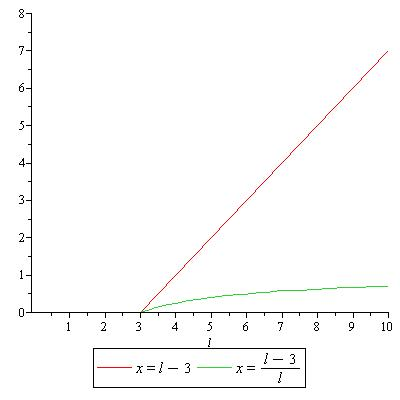
\includegraphics[width=0.5\columnwidth]{ChapterABM/figures/coremodelprodABMjpeg}%
\caption{Core model production function showing total output and average output per unit of labour}%
\label{fig:coremodelprodABMjpeg}%
\end{figure}

Only positive values make sense in an economic context, and as can clearly be seen, the fixed labour requirement means no production is possible at all unless three units of labour are input: an indivisibility. This is straightforward enough to impose analytically, but how might it work in an agent context? The answer is a useful illustration of how rationality, timing and `\gls{blindsearch}' interact. Consider these two possibilities:

\begin{enumerate}
	\item Actors decide sequentially, looking at what firms are producing in order to choose whether to work;
	\item At $t-1$, Actors randomly choose a potential employer. If at $t$ this was successful, they repeat the same action. 
\end{enumerate}

The first of these assumes actors are able to rationally choose a workplace. However, each actor is only able to contribute one unit of labour; a firm needs three to even begin producing. The rational result is that no work takes place and nothing is produced: the model cannot get started. The second is the most rudimentary \gls{blindsearch} possible: attempt some random action at one point in time, and see if it improved things on the next day. If it did, stick with the same strategy. Even with a set of actors consisting of only four people and $n$ firms, given enough time they would all randomly find themselves selecting the same firm and allowing production to take place.

Note, this is not really `blind search versus rationality' as such, since the search requires actors to have the most fundamental attribute required for rationality: to be able to tell `better' from `worse'. 

%WUD 40	Blind search agents: advantage = they have no need to know everything at the same time. Attempts to improve position can be separated out over many timesteps.

%WUD 43	Brute force vs analytic optimisation: catch 22 in actor model where they try to optimise on their time-step: no stock = no point in working; no work = no stock.

%%%%%%%%%%%%%%%%%%%%%
% COMMUNICATING COSTS
%%%%%%%%%%%%%%%%%%%%%
\subsection{Communicating costs \label{sec:comm_costs}}

The first technical challenge is dealing with price. In the \gls{coremodel}, a numeraire approach is used, as described in section \ref{sec:keyconcepts_coremodel}. The `price' of the agricultural good is designated the numeraire. Because output is linear, workers are always `paid' exactly the same. Compare what would happen if numeraire output has increasing returns: output per worker would be higher for larger worker input, and the value of the numeraire would change accordingly. So, any complications regarding agricultural wages are thus done away with. The analytic advantages for the \gls{coremodel} are strong. When it comes to building an agent model with more than one good, however, the numeraire approach is difficult. The existence of agents requires the modeller to specify the relationships between them explicitly: there is no avoiding it. If, for example, two firms each make a different good, and one is the numeraire, each firm must pay wages in that numeraire. How does the non-numeraire firm do this? It must acquire the currency, and can only do this by exchanging what it produces - yet there is no guarantee the numeraire-producers want to exchange. In the basic \gls{coremodel}, for example, no manufacturing output is required to produce agricultural output. An explicitly coded numeraire, then, seems unworkable on the face of it.
%I will try and build one that avoids money, but that's a little way off: it'll be back to collaboration again, plus Edgeworth-like trading.

The use of fiat money solves this problem: all goods and wages can then have a negotiable price. However, a whole set of new challenges accompany the use of money. 


Exchange of information between humans is not the same as for `information' in a computer, or in genes for that matter.  There's a symbolic system: ``The information held and transmitted in the form of a symbol is thus embedded in a network of interconnected meanings, related to and produced by social structures.  Genetic or computer information does not have this quality; it is at most indexical. In contrast, human information is structured and cultural; it is entwined with institutions.'' (\citealt{hodgson_economics_1996} p.253)



\begin{comment}

E.g Eos: (MM2 43) Firms should be able to exploit EoS, but how should that happen? Cf MM1 42 backyard.
MM1 66: firms with higher inputs of labour should have an advantage - they should be able to find a better price than others, if they're ahead; they should have able to get a monopoly.

The point there: geneq is meant to do this; account for all those dependencies. Cf. Fowler.

WUD 4	``Although a full description of this alternative is beyond the scope of this article, it appears that the choice of asynchronous rather than synchronous decision-making is not a key point in understanding the differences between the agent-based and analytic models.'' (Fowler 274)
I disagree! Big, complex issue. Order and randomness large effect on outcomes. Maybe not so with Fowler's very small number of agents.

WUD 22	Auctions vs on-line adjustment versus simultaneous eqs. Actors' decisions spread over time = normal.

FDA 16: Trapped in loops of dependency! Where to work, what to buy, who to hire, where to locate? All affect each other. 

Update: I should just note quite how much I struggled with this problem initially. The answers wer far, far from obvious. I have a solution that runs, but a) many more must exist and b) it may run, but does it really work?

Quote from Fowler: ``the amount a firm can offer in wages is dependent on the amount it can produce and price it receives for its goods. These quantities are affected, in turn, by consumer's wages, which depend on which firm employs them (and whether or not they have found employment at all.)'' (p.277)
There's intrinsically a limit on what agents can do to solve these problems. There's game theory: trying to optimise under uncertainty. But it's not a problem of lack of information: it's a problem of incalculability. 
This may mean, also, that - say - the resulting number of firms is due to a random number failing; no way to predict who, but the incalculability of the problem means that only some will make the right guesses. Cf. Baumol quote on what firms should do to optimise.
Also noted here that the landscape itself is a form of memory.

From Oeffner:
Incalculability: p.25. He talks about it in different terms, but it's the same issue: a difference between 'risk' and 'true uncertainty' stemming from the fact that you don't know what other agents are going to do. Ties to data, meaning
'Endogenous uncertainty': Pesaran 1987. On p.27. That's exactly the problem with two firms trying to find a good location. 


FDA 17	Agents deciding when to sell. Fream: farmers releasing goods in a way that smooths prices. Cf. Kirman's argument about the representative agent, and disaggregated models explaining this kind of smoothing.
The point there isn't so much that you can affect demand - you can, but the effect is small - but that you want to adjust your timing to fit with the macro-effect of supply on demand. You can't really affect prices, but you know prices are going to change in a certain way over time. So, you're a price-taker in the short-term, but there's a longer-term strategy that means you have some wiggle-room - so are actually not a price-taker - and the long-term result is a smoothing of prices. Again, Kirman.

WUD 1	Fowler: ``it is impossible for firms to make decisions about production levels without knowing exactly what every other firm will do and where labour will be available.'' (p.265)
But they don't need to: blind groping. 

WUD 1	Common goal of 'perfect information' vs 'groping' agents: optimisation. Question: how important, if at all, is the 'realism' of the agents? Mine aren't at all. One arg: objective existence of optima; nature of agents doesn't matter; disaggregation is the thing. Fowler: : ``Agent-based modeling works by disaggregating the modeling environment to the extent that each firm and agent is represented as acting individually.'' [265]

==
WUD 2	Determinacy, uniqueness, stability. Necessary for equation-based results? ABM: randomness = come up with probabilistic answers. 
WUD 3: Useful quote, Fowler: ``The economy as it has been represented in geography is typically far too chaotic to be considered at rest or to be operating at some market-clearing point where all labor is employed, all production is consumed and utility is maximized (Plummer et al., 1999).'' (p.271-2) No-one claims that the real economy will reach a rest point, only that the models help us understand the equilibria it moves towards. Think ball on rubber sheet in high wind.
Plus, if completely blind agents can find their way "on-line" to optima, that chaos doesn't present a problem. May be too chaotic to be at rest, but not so chaotic that optima can't emerge through blind luck (and not evolution, unless one considers the landscape as an evolutionary memory. If so, it's Lamarkian!)
There must be a trade-off between how much the world is changing and how much blind groping can achieve, and it must relate in some way to this point about equilibria and change. God knows how though.  
Plus, do agents only capable of telling better from worse count as rational?
WUD5: If a model can grope it's way to optima, with agents' only ability being that they can compare 'before' to 'now', what does that say about the economics? I think this: the equation approach is still entirely valid, but perhaps it's not describing micro-motives. Perhaps instead it's illustrating where the optima are and nothing more. The appeal to utility as a mechanism is false: no action is taken to reach that optima.
One might argue against that: if it can be shown that agents can indeed reach those optima through groping (cf. Walras) then we can assume the mechanism and continue to use analytic optimisation. I'd reply: you have to show that the mechanism does, in fact, work. 
update: which is Epstein's point...
==

MM1 8	Granular, on-line, no market clearing to be done. The many many uses of blind groping.
MM1 15	Supply and demand: stochastic, iterative, not 'clearing'.


===
MM1 18-	Write-up of optimisation and GA. Most useful algorithms assume that there will be some correlation between the quality of 'neighbouring' candidate solutions - those close in the space. Genetic algorithms assume that high-quality 'parent' candidate solutions from different regions in the space can be combined via crossover to, on occasion, produce high-quality 'offspring' candidate solutions." [Mitchell GA p.7]
"What is maximising on-line performance good for? Holland's view is clear: the rough maximisation of on-line performance is what goes on in adaptive systems of all kinds, and in some sense this is how 'adaptation' is defined." [124]
On-line performance: stealing that idea. That was previously "live groping!"
Satisficing.
Worth-noting: GAs combined with hill-climbing algorithms often found to work better than GAs alone. [124] Would seem very likely to be the case for my agents. "GAs seem to be good at quickly finding promising regions of the search space, and hill climbers are often good at zeroing in on optimal individuals in those regions." [124]
Cf. MM2 73: "crawling around in utility space, possibly attempting to swim up a too-turbulent stream and not finding their way�"
===
MM1 42	Cf. split decisions of beanworld; separate auctions for work time and bean buying.
MM1 42	Contrast: backyard model, where actors are able to immediately know whether a particular decision will be more productive for them; indeed, the decision can be taken to be the production, it's so simple. Not so here: the EoS necessary to ultimately lower the cost of production can't happen without a number of people working for a firm; yet, that won't happen below a certain critical theshold, or possibly can't happen at all, given the way I've coded it.

MM2 65	Discussion: the more blindly agents can find optima, the more one can say the objectively exist? Cf. fact the agents make the world they're optimising in, so it can't really be objective can it?

MM2 73	Details of person action choice 2, random groping. So, they might try wage - thus producing stock, thus breaking out of catch 22.

MM1 15	The trick: actors deciding "as if" others are still contributing their time. Need to write up, perhaps compare to simple game theory example

===

MM1 41	Stock running out for some firms shouldn't mean they can't hire - if they have the money. Cf 2 optimisation choices and problems.
MM1 42	Does the stock-crash end-of-model problem say anything interesting about the real world? Is it anything like a co-ordination problem? I.e. people want work, firms want to sell goods, catch 22?
Breaking out: letting work happen before stock levels are known. Is this just a practical modelling solution or something about the real world?
MM1 42	Cf. split decisions of beanworld; separate auctions for work time and bean buying.
MM1 42	Contrast: backyard model, where actors are able to immediately know whether a particular decision will be more productive for them; indeed, the decision can be taken to be the production, it's so simple. Not so here: the EoS necessary to ultimately lower the cost of production can't happen without a number of people working for a firm; yet, that won't happen below a certain critical theshold, or possibly can't happen at all, given the way I've coded it.

%%%%%%%%%%%%%%%%%%%%%%%
% Pasted from Framework: belongs here?
%%%%%%%%%%%%%%%%%%%%%%%

\end{comment}



\section{Production and utility in an agent context \label{sec:produtility_agents}}

\begin{comment}
Contrast to what agent firms need to do; data, meaning�
Cf. Baumol: faced with a particular reality, what sort of theory is actually going to help firms succeed?
"It is at least possible that shear business acumen and experience permit management and other economic units to arrive at decisions which come close to being optimal. Moreover, in business, competition may soon eliminate firms whose decision-making is consistently poor. To the extent that these assertions are valid, optimality analysis should serve as a relatively good predictor of economic behaviour; that is, it should provide a reasonably good explanation of actual economic decisions and activities." [5]
Plus, randomness, sequence, luck may also eliminate a certain number. 
Cf. nature of optimisation; function standing in for process of groping, etc.

\end{comment}

%%%%%%%%%%%%%%%%%%%%%%%%%%
% OUTLINING UTILITY BEING USED IN MY MODELS
%%%%%%%%%%%%%%%%%%%%%%%%%%
\subsection{Using utility in an agent model \label{sec:rationality}}

In the model framework developed for this thesis (described in detail in chapter \ref{chapter:modelfw}), agents use a set of `standard' utility functions. The functions themselves have been covered in the previous chapter. 

Many agent-based critiques of economics argue that the utility-maximising approach is an unrealistic straight-jacket... blah. This section argues in support of using utility. If understood properly, and used with awareness of its limitations and meaning, utility-maximising agents are a very useful tool.

One of the central criticisms of utility theory is that people are simply not like that. (x-ref Edmonds.) This is examined in more depth below, but it is useful to quickly explain the thesis' position on this: people are not utility-maximising automatons, but utility theory \emph{is} a useful way to analyse how people react to changes in costs. There is no need to make any sophisticated case for the psychological basis of utility; it can still be used as a modelling tool. Neither does this mean more sophisticated models of behaviour are unimportant: utility is merely a simple, effective way of gaining insights into the impact of cost changes. There are some pitfalls to be avoided when interpreting utility-based agents; these are discussed below.




Some things I need to cover:

utility as tautology / hedonistic / actual internal description of psychological state. Problem of information, uncertainty. The point about realism.

What's the value of realism?

A defence of the use of utility requires understanding what the type of agent model developed here is being used for -  what it is being asked to do. [does it? That's nice.]



The basic point is that utility provides a relatively simple way of describing how people react to changes in cost. It does this job admirably - but problems arise when.. when what? 


In theory, no more need be said on the matter; in practice, more justification is required, since much confusion arises from its use.


Bouncing off Einstein's almost cliched quote; the surprise that nature should be so describable by maths. The description has so much veracity, it's possible to forget that it is 

The tight fit, the close isomorphism, between reality and physical models means we trust those models to predict, we trust them with our lives. But it still hides the basic truth that physical models are still only a description, a way of representing reality. Map and territory are not the same thing. Forgetting that fact causes much confusion when it comes to modelling in the social sciences. In particular - and this is Friedman's point - there is a belief that physical models closely match actual structures in reality and that's where their power comes from. Of course that isn't true: they massively simplify reality, for example by treating planets as points. Adding more `realism' makes many models worse, not better. 

This is a problem for \gls{ABM} because, oddly, their ridiculousness is more visible. In reality, firms do not crawl about on a 2D plane, people do not hop effortlessly from place to place searching for the most utility. 

\subsection{Very brief history of utility}


\subsection{Is utility `credible?'}

The work of Moss and Edmonds is a good example of a general view within agent modelling: the `standard' economic approach to modelling people using utility is simply not `credible'.

1. Thomas Brenner, Computational Techniques for Modelling Learning in Economics (Springer, 1999).
That's got this PDF: http://cfpm.org/cpmrep33.html. Also in zotero. 

See also: 




\subsection{Utility as empty tautology}

Compare two examples of the use of utility from the literature: one from transport economics, the other from rational choice theory. Approaches to utility in transport economics have used the idea of revealed preference successfully to say useful things about people's choices. Button points out that - 

"the general conclusion about the idea that some overall budget mechanism governs individual travel decisions, however, must be that, to date, the evidence available still leaves many questions unanswered and the theory is still largely unproved." [92]

Yet, despite this, many directly practicable ideas have emerged through trying to understand how people react to cost changes. One that stands out is finding revealed preferences for travel time: ``if a person chooses to pay \$x to save y minutes then he/she is revealing an implicit value of time equal to at least \$(x/y) per minute.'' This has led to - 

``savings in walking and waiting times are valued at between two and three times savings in on-vehicle time - parameters that have proved to be remarkably robust over the years.'' [104]

This is striking: how people value travel time is not simply a function of the time taken. Those willing to commute by car for an hour each way would be much less likely to walk that distance. As regards this thesis, the crucial point is that no argument need be made about the underlying mechanism or the rationality of those making a choice between walking or driving to work. There is, of course, value in attempting to understand what underpins those choices, but equally there is value in accepting and applying the finding. The underlying causes may be complex, but this does nothing to lessen the importance of the result itself.
%Survey: Walters, 'value of travel time saving used in road project evaluation: a cross-country / jurisdiction comparison', Austr trans reserach forum 92.
%Paper: Hensher - 'measurement of the valuation of travel time savings', journal of transport economics and policy, 2001
%From a Leeds study, think this might be the one Varian talks about. Quarmby, 'choice of travel mode for the journey to work: some findings', journal of transport economics and policy, 67.
So people willing to commute for an hour each way would be much less likely to walk that distance.  Utility describes but does not explain this.

Compare this to rational addiction theory...

Blaug On samuelson's revealed preference theory (RPT): ``provides a perfect example of our earlier contention that the logical distinction between `assumptions' and `implications' disappears in a perfectly axiomatized theory.'' [143]



The problem is simply enough stated: if any outcome can be described as rational, then the theory is completely unfalsifiable. 

But it depends on what you're falsifying, and what you're able to falsify with the theory. Any description of gravity that we have isn't really in a position to falsify the graviton theory. It'd need some deeper level of data to uncover what's going on. 

The physical analogy can only be taken so far, of course: in reality, there are plenty of ways of showing that people are not utility maximisers. The argument for using utility must, therefore, be relatively lightly made: it is a useful tool, as long as its limitations are kept in mind.


%MM1 20pp/23	Reasoning behind bundle approach; cf. to Fowler's 'objective demand' approach. Write up.
%%%%%%%%%%%%%%%%%%%%%%%%%%
% OUTLINING UTILITY BEING USED IN MY MODELS
%%%%%%%%%%%%%%%%%%%%%%%%%%
\subsection{Rationality n ting \label{sec:rationality}}

The goal of agents in these models is the same as those in \gls{ge} - to optimise either their output or their utility. The technical challenges of achieving this in an \gls{abm} setting, however, prompts some useful questions. This section looks more closely at the nuts and bolts of getting agents to optimise.
%The process of developing the models led to a number of unexpected issues; these are a very useful way to analyse the fundamental differences (and similarities) between agent and analytic modelling approaches.

Section \ref{sec:frameworkUtility} in chapter \ref{chapter:modelfw} explains how utility is used in the model framework. This section outlines the key ideas that led to those model choices. The central issue stems from problems using `objective' utility function optimisations of the type explained in section \ref{sec:utilityintro}. In these, a utility function is constrained by a budget. This produces a set of equations giving the `objective' optimal quantity of goods, given that budget. The approach in  \gls{ge} (and many other economic models) is to assume the objective demand implies the correct level of production to meet it, and thus the correct number and scale of firms. In terms of agents, as Leijonhufvud puts it -

%http://www.forvo.com/word/leijonhufvud/ Lay-on-huh-vud.
%constrained optimisation models attribute \emph{substantive rationality} to agents. Thus, 
\begin{quote}
``in this theory utility or profit maximisation is a statement about actual performance, not just motivation... The theory does not leave room for failures to realise the relevant optima.'' (\citealt{leijonhufvud_agent-based_2006} p.1628)
\end{quote}

%In discussing `market design' using agents, Marks points out that building artificial markets has forced programmers and theorists to move away from closed-form equilibria. (\fixref{Marks chapter in handbook}) More specifically
This is not just an abstract criticism of the constrained optimisation approach: it is a problem that needs solving in agent models using utility. Fowler's approach is to make a tactical choice to allow agents their objective demand. As he puts it, ``workers select their optimal bundle of goods without reference to the actual supply of the good'' (\citealt{fowler_finding_2010} p.10). This avoids the need to solve rationing of limited goods. It also sends ``clear signals to firms about the actual level of demand for their goods at the current price'' (ibid).

As has been argued, \cmt{where argument about conscious defence of model sillinesses?} all models will have implausible-appearing assumptions, and it is the job of the modeller to consciously acknowledge what they are, and justify the analysis that includes them. The job Fowler set himself was to stick as closely to the \gls{coremodel} as possible, and keeping objective demand is a part of that. This thesis takes a different approach. 

---
%%%%%%%%%%%%%%%%%%%%
% PRODUCTION AND EOS
%%%%%%%%%%%%%%%%%%%%
\subsection{Coordinating simple production \label{sec:coord_production}}

Section x explained that, in the \gls{coremodel}, firms have a production function that gives them increasing returns from labour input. It was also noted that those increasing returns are analysed away: changes in welfare through production come about solely through changes in the equilibrium number of firms, and thus the total number of varieties consumed. 

But Leijonhufvud's point applies here too: analytic approaches skip to the end of the process of production. They describe optima, and build that description on an explanation devoid of specific actions to get there. Whether or not this approach is justified (a point discussed more below) is beside the point when it comes to building an agent model of production: \gls{abm} applies its own restrictions here, forcing the modeller to work with specific `Firm' agents, and specifying what actions they must take in order to manage production. (x-ref Fowler discussion.) As just mentioned, firms enter and exit the market also. An agent approach must decide how to address this, even if to explicitly avoid it. 

So the question is: how to build Firm agents? What are the issues? In both the case of Firms and People, this thesis has attempted to build the simplest basic economic behaviour into them (and also agrued this is justifiable). 

The most obvious starting point is to ask, what are Firms' goals? Their over-arching aim is simple enough to state: maximise net revenue, which is gross revenue minus costs. If a Firm can stay afloat doing this, they can survive. This simple aim quickly becomes complicated when considering all the options then facing a model of Firm action. Chapter \ref{chapter:modelfw} explains in detail what options are examined in this thesis, but now is a good time to explore the over-arching issues.

Section \ref{sec:fowler} discussed Fowler's eloquent encapsulation of the co-ordination issues involved: 

``the amount a firm can offer in wages is dependent on the amount it can produce and the price it receives for its goods. These quantities are affected, in turn, by consumer's wages, which depend on which firm employs them (and whether or not they have found employment at all.)'' (\citealt{fowler_taking_2007} p.277) 

This tangle of dependencies can be broken down to see how each element in an agent model might relate to each other. Firms can be modelled in ways that avoid many coordination issues, while still helping to shed light on the modelling problem. One approach is to break the cycle of dependencies completely. By providing People with a fixed wage income every turn, issues of money circulation are avoided: firms do not need to set or pay wages, and so payment can appear and disappear again in one day without the need to circulate.
\cmt{need to x-ref with numeraire stuff / ways to solve money problem / meaning of money etc. Maybe.}
%Diagram showing this? E.g. flow vs "`in >> person >> firm >> out"'




%%%%%%%%%%%%%%%%%%
% ARE BLACK BOXES TELEOLOGICAL?
%%%%%%%%%%%%%%%%%%
%\subsection{Are black box models teleological? \label{sec:blackbox_tel}}

Hayek, in his short essay, `the use of knowledge in society' (\citealt{hayek_use_1945} p.529) criticises Schumpeter for using ``objectively given quantities of commodities impinging directly upon each other, almost, it would seem, without any intervention of human minds''. Hayek quotes Schumpeter as arguing that -

\begin{quote}
``... the possibility of a rational calculation in the absence of markets for the factors of production follows for the theorist `from the elementary proposition that consumers in evaluating (`demanding') consumers' goods \emph{ipso facto} also evaluate the means of production which enter into the production of these goods.' '' (\citealt{schumpeter_capitalism_2010} p.175 in Hayek, ibid.)
\end{quote}

\cmt{this crosses over with args about monocomp, e.g. in Fowler section.}

The first thing to note is that this is an argument made by \gls{ge}: production is assumed as the mirror image of consumption, and everything else about firms, including their equilibrium number, flows from that. \footnote{There is a classic Hayek quote here: ``the problem is thus in no way solved if we can show that all the facts, if they were known to a single mind (as we hypothetically assume them to be given to the observing economist), would uniquely determine the solution; instead we must show how a solution is produced by the interactions of people each of whom possesses only partial knowledge. To assume all the knowledge to be given to a single mind in the same manner in which we assume it to be given to us as the explaining economists is to assume the problem away and to disregard everything that is important and significant in the real world..'' (\citealt{hayek_use_1945} p.530; see e.g. \citealt{miller_complex_2007} p.87)}; the important part for the argument being made is that Hayek believes Schumpeter to be ``disregard[ing] everything that is important and significant in the real world'' (ibid p.530). 

%(which is kind of Krugman's argument) 
What does he mean? Jacobs has another example that may help to illustrate the point. She attacks arguments that comparative advantage originates from the division of labour as teleological; ``one might as well say rain is beneficial to plants and that that is why it rains.'' (\citealt{jacobs_cities_1986} p.70) For Jacobs, as well as Hayek, the logic of causation is wrong. As she says, of the definition of efficiency intrinsic to increasing returns: ``to say that the economy of Uruguay... was more efficient because more specialised than the economy of Switzerland is to stand reality on its head'' (ibid p.71). Jacobs wants to build a causal argument about the role of `nests of symbiotic suppliers'; any black box approach makes this impossible. Above, however, it was argued that treating economic entities as black boxes is acceptable, depending on what argument is being made. So what is the problem? 

The reason this point has been laboured is because it transpires there are very specific ways in which Hayek and Jacobs are correct: when the problem of production in space is posed from actors' points of view, several of the key functional assumptions of constrained optimisation cannot work. Some `black boxes' can still be used, however, and the issue is not quite as clear cut as Hayek's job-lot dismissal would imply. The devil is in the detail, however.

---

%%%%%%%%%%%
% Brute force vs analytic
%%%%%%%%%%%
%As discussed, the two-good models use an `Engel function' able to either act as a Cobb Douglas if $\gamma$ is set to zero, or to distinguish the two goods as necessity and luxury (see section \ref{sec:utilitynengelslaw}) . 
%In an analytic setting, using  constraints (equations \eqref{eq:engelsmurataFopt} and \eqref{eq:engelsmurataFopt}) would be normal. 
As discussed above, for a given budget and set of prices, equations can be deduced that say precisely what the optimal quantity of goods should be. In an agent setting, it is possible to find optima through brute computational force: simply search the entire parameter space and keep whichever produces the highest utility. This is, of course, more computationally expensive than using a simple constrained optimisation equation, so it is a natural step to wonder whether those equations can be used instead of a brute force approach. The answer, surprisingly, is no. 
%Section \ref{sec:blackbox_tel} picked up on some of Hayek and Jacobs' arguments that gave a background to why this might be so. Here, some modelling reasons that support their argument are discussed.

Consider three options for an actor finding its maximum utility - brute force, or one of two constrained optima, the first constrained by a given total quantity of the two goods, the second including the price of both goods. In the brute force approach, the actor searches a range of possible mixes of $F$ and $M$ in Cobb Douglas utility function \eqref{eq:-3} to find the optimal mix:

\begin{equation}
max\; U=F^{\delta}M{}^{1-\delta},\; (0<\delta<1),\; F+M=Y
%U=F^{\delta}(M+\gamma){}^{1-\delta},\; (0<\delta<1),\; \gamma\geq0,\; F+M=Y\label{eq:engelsmurata2}
\end{equation}

As discussed earlier, for a budget of $F+M=Y$, the non-price constrained optima for the two goods is:

\begin{equation}
F=\delta Y
%F=\delta(Y+\gamma)\label{eq:engelsmurataFopt2}
\end{equation}

\begin{equation}
M=(1-\delta) Y
%M=Y-\delta(Y+\gamma)\label{eq:engelsmurataMopt2}
\end{equation}

Including price, the optima are as follows ($p_F$ and $p_M$ are the price of $F$ and $M$ respectively).

\begin{equation}
F=\frac{\delta Y}{p_F}
%M=\frac{Y(1-\delta)}{p_{M}}-\delta\gamma\label{eq:engelpriceoptM}
\end{equation}
 
\begin{equation}
M=\frac{(1-\delta) Y}{p_M}
%F=\frac{\delta Y-Y+\delta\gamma p_{M}}{p_{F}}\label{eq:engelpriceoptF}
\end{equation}

So why can't either two of these constrained optimisations be used? It is impossible to assume that goods will be available to meet a set `objective' demand. Consider what people must do (outside of the choice of backyard, which avoids all co-ordination problems.) They need to find information. Either -

\begin{itemize}
	\item How much of F or M can I get for my time?
	\item How much money can I get for my time, and how much of F and M will that buy?
\end{itemize}

Even if time or money can be used to produce an `objective demand', the model probably cannot supply it. The only option for people is to check what bundles of goods are available and test which mix is best. Compare this to equations \ref{eq:engelsmurataFopt2} and \ref{eq:engelsmurataMopt2}: both require prior knowledge of the budget, $Y$ - that is, the total quantity of goods. That `budget level' is not given - there is a wage, but not an `amount of $F$ plus $M$'. 


%%%%%%%%%%%%%%%%%%
% BLACK BOXES 
%%%%%%%%%%%%%%%%%%
\subsection{`Black boxes' in production and utility \label{sec:blackboxes}}

Er, what was I going to say here?
%%%%%%%%%%%%%%%%%%%%%%%%%%
% CUTTINZ
%%%%%%%%%%%%%%%%%%%%%%%%%%

%While Solow and Krugman are in large part correct, there are problems  with their case. Most fundamentally, there is a large gap between, say, Krugman's stated awareness of a model's ``silly assumptions'' and the uses to which those models are now being put in policy circles. 

%Pursuit of that argument, however, is beyond the scope of the thesis. The more important issue at hand is this: there are implications for agent modelling. How so? It comes back to Daly's claim that standard economic functions offer only 	 (p.262) Consider an agent model of production that has aspirations to examine the complex morphology of linkages seen in reality - Jane Jacobs' `tangled bank'. Agent models are almost always explicitly time-driven; computer cycles are synonymous with timesteps and iteration is central. In such a world, what moves between economic linkages each timestep, if not actual resources? Certainly, many exchanges can be service-related, but in a time-driven model it becomes much harder to conceive of resources in an abstract away. Instead, a more Weberian image presents itself as the most likely: resources with weights, combined to produce other resources with weights.

%Trying to think this through. It seemed important to me because I can't get utility functions to work in an agent context. But then in what circumstances am I saying its OK to use increasing returns? This might be better in that section.
%Her answer: "economic forces originating in import-replacing cities shape economic life outside of cities... when the force at issue is the power of a city market bearing upon regions that lack import-replacing cities of their own, the results are specialised regions." [70]
%She also argues with the definition of efficiency intrinsic to narrow EoS: "to say that the economy or Uruguay, 'the Switzerland of South America', was more efficient because more specialised than the economy of Switzerland is to stand reality on its head." [71]
%And, of course, it's right  - I think. I'm just mulling over the weird role of the theory of comparative advantage. It purports to describe, but it also underpins a prescription: opening up to trade capitalises on comparative advantage. But where does it come from in the first place? In krugman, it's just a function of input. But - as Jacobs rightly points out - that tells us nothing about its actual origins.

%%%%%%%%%%%%%%%%%%%%%%%%%%
% CRITIQUES N TING
%%%%%%%%%%%%%%%%%%%%%%%%%%
%Jane Jacobs' arguments present a good critique for the straightforward  'black box' model. Where the point of those models is that an in-out relationship can be defined - and only altered through some technological change - Jacobs' description of production paints a picture of economic actors stumbling upon new combinations of goods in a way very reminiscent of evolution. 

%Perhaps the most challenging productive factor to theorise is knowledge. An example from Krugman illustrates the sort of interactions that can take place. He argues that as energy became cheaper and more accessible, it could substitute for skilled labour. The result was a replacement of that labour by cheap energy sources - and an increase in the footloose mobility of workers, because pools of local skilled labour were now less necessary. 

%Structural vs input factors




\section{Space, networks and market structure \label{sec:ABM_networks}}

Explicit space imposes two related issues onto agent models. The first is that `clearing market' conditions do not hold. As Leijonhufvud puts it quoting Hicks -

\begin{quote}
``In a normal, ongoing market, transactors are not all brought together in a single location and at the same time. Without centralisation and synchronisation, the supply-equals-demand condition `cannot be used to determine price, in Walras' or Marshall's manner'.'' (\citealt{leijonhufvud_agent-based_2006} p.1633)
\end{quote}

%``Instead, ongoing markets require market makers who announce their prices and maintain inventories to handle customers arriving at irregular intervals." What I'm calling a granular market to contrast to the clearing one.''
It is possible to circumvent this fact if all economic actors are presumed to exist on a point - but explicit space rules that out. It follows that actors cannot make decisions simultaneously, in a way that could lead to `clearing'. Markets designed to clear can exist in space, but these are not the norm; instead, the market is made up of decisions made at ``irregular intervals'' (Leijonhufud, ibid.). When building an agent economic model in space, this is a fact that quickly becomes apparent, and some work needs to be done to define the range of options to deal with it. 

The second, related condition imposed by explicit space is that actors naturally form networks. Take the most basic example from section \ref{sec:spacenutility}, which outlined the simple rule \eqref{eq:circlerule} defining the set of actors' neighbours simply as `others within a given radius'. Actors face overlapping groups of potential trading partners: as well as making it impossible to assume that all prices can be simultaneously adjusted, as just discussed, this can be used to define a network.

This form of spatial graph has been studied in both discrete and continuous forms, and in an agent context.
\cmt{Think I'll wait on these refs to see what I write next...}

The theoretical existence of these network properties is not always relevant to model outcome. In the backyard model in section \ref{sec:backyard}, for example, while actors have the option each turn of deciding on a collaborator, one central site quickly becomes locked in. As soon as this happens, any potential network effect disappears. In more complex models, however, the network structure becomes more important. The density of actor networks within possible travel radii is the foundation for cost signals. In this context, agglomeration and space cost changes will impact on these network effects by moving the model towards stronger synchronised signalling. 

%Networks connect to diffusion, of course: so, price signals, demand signals may diffuse. 1D model perhaps best for trying to trace how that works.

%As Ladley and Bullock point out, an immediate consequence of economic actors having explicit location is that `single market' assumptions no longer hold (\citealt{ladley_effects_2007} p.83-4). Most obviously, a `clearing' model of market action will not work: 

%So I model granular agents; I've written about that, possibly in zotero notes for the last comp handbook chapter.





%%Notes on section: I think I should x-ref to where I discuss Fowler in more depth. E.g. where I'm talking about the nature of objective demand. 

%\section{Fowler [better name needed!] \label{sec:fowler}}

Christopher Fowler (two papers here) has attempted to recreate the core model in agent form. It is useful to consider the approach he took and the obstacles discovered along the way. Fowler firstly attempted to take the core model out of its equilibrium assumptions; an agent approach, he argues, is a good method for achieving this. He set himself a specific goal: to ``re-create as exactly as possible the relationships in the economic [core] model'' (p.266) in agent form, meaning that ``to the extent possible, the equations used to express the analytic model have been maintained.'' (p.272) Fowler's direction of travel, then, is very much from the analytic core model towards agent modelling. For instance, he keeps the final set of simultaneous equations outlined in section \ref{sec:coremodelapx}. The main conclusion from his first attempt was that -

\begin{quote}
``although the equations of the analytic model can be mimicked in a way that is sufficient for a simulation to run, such a simulation cannot be made logically defensible without significantly altering the relationships among workers, firms and cities posited in the analytic model.'' (p.282)
\end{quote}

In initially binding himself to the assumptions of the analytic core model, Fowler was stuck with one of the more thorny abstractions: there are no firms explicitly defined. The equilibrium number of firms - a key feature of of the Dixit-Stiglitz \gls{monocomp} approach, as discussed in section \ref{sec:marketstructure} - is purely a consequence of consumer demand combined with love of variety. As he puts it, ``firms appear and disappear in cities based on the full employment of the workforce even to the point of following the lead of workers who move from place to place in order to benefit from increased real wages.'' (F2 p.2) 

\citealt{fowler_taking_2007} defined firm agents, but in sticking with the analytic model's mechanisms, avoided defining any mechanism for matching firms to workers. Following their own motivations, ``when firms move, they tend to want to move to places where wages are low; in contrast, workers tend to want to locate where wages are high'' (\citealt{fowler_taking_2007} p.276). 

Fowler's first pass at an agent version of the core model, then, lacking any method for linking firm and consumer behaviour even implicitly, could not produce equilibrium firm levels. Fowler notes that ``as a result, the model fails to move towards any of the equilibrium conditions predicted by its analytic counterpart.'' (p.266) In his second paper, Fowler attempts to address this by defining mechanisms, having already identified a list: 

\begin{quote}
``firms would bid for labor through wages and set prices for their goods at a level where they would expect to make the greatest profit. Workers would then consume based on the available prices and quantities; utilities and profits could be calculated for all agents. What sets this type of specification apart, however, is that it would make no assumptions about individual firms making the correct choices. Firms that chose correctly would be rewarded, and those that chose poorly could be dropped from the model.'' (\citealt{fowler_taking_2007} p.280-1)
\end{quote}
%The equations for things like production and wage would be truly independent rather than derivative so the model could handle a wide range of parameter configurations. 
%Actors with motivations, mechanisms connecting them and a variety of assumptions about the dynamics that these two together will produce. Fowler suggests some of the mechanisms that a full agent version of the core model might do: 

This is a fully agent-based picture he paints: each actor making decisions entirely independently, based on the information at their disposal. Fowler goes on to say, ``as complex as this specification sounds, it is actually relatively simple in an agent-based framework where bounded rationality, learning by doing and other types of decision-making all have substantial supporting bodies of literature.'' (ibid.) 

Not so simple. How to say? Break the problem into two components: first, how actors make decisions; second, whether they can collectively coordinate their actions into globally desirable economic outcomes. That, in a nutshell, is the `general' problem in general equilibrium analyses. 



Fowler discusses some of the dependencies that must be solved if an agent model is to work: ``the amount a firm can offer in wages is dependent on the amount it can produce and the price it receives for its goods. These quantities are affected, in turn, by consumer's wages, which depend on which firm employs them (and whether or not they have found employment at all.)'' (\citealt{fowler_taking_2007} p.277) 


Creating a functioning agent model of work and consumption can often involve making coding compromises. Fowler's approach to consumption reflects this: a tactical choice is made that avoids the need to consider rationing of limited goods. As Fowler puts it, ``workers select their optimal bundle of goods without reference to the actual supply of the good.'' (f2 p.10) Thus, they still have an `objective' demand level. He notes a key informational advantage: this sends ``clear signals to firms about the actual level of demand for their goods at the current price'' (ibid.) 
%I do the same currently: infinite stock. 

This reflects the prime difficulty of producing coordination in an agent model of this sort. A proponent of the analytic approach to the core model might argue that this demonstrates the power of the analytic method, but this misses the point Fowler's work has made. Just because dynamics of coordination are hidden behind equilibrium assumptions does not mean they have gone away. It is still very much an open question: how can actors, unable to coordinate through any central mechanism, produce stable spatial economic outcomes? Indeed, is there a model than can achieve this, or are there reasons to believe it might not be possible?
%Referring to the metis arg here. Analytics may describe and endpoint, but the metis argument rules out being able to produce a model of the process. Discuss!



Notes the 'absence of rational expectations' (p.275) - ``The firm and worker agents have perfect information in the sense that they can know the outcomes of their decisions up to a point, but the simulation environment is dynamic and the conditions that they observe at the time they decide where to move will not remain constant as other firms and workers make their own decisions.'' (p.275) Discussed much here in relation to what rationality means in an agent context. Do my blind agents, able only to know when a random grop improved their lot, count as rational?


Later: ``To create such a model, firms would have to have some mechanism with which they could predict an appropriate production level for themselves and estimate the levels chosen by their competition in an environment where sufficient labor supply is not guaranteed. The delicate balance among the equations of the analytic model does not allow for the error and uncertainty that are necessary parts of this sort of prediction, and so a new set of relationships needs to be specified.'' (p.282)
He notes that analytic choices made to gain tractability can ``actually make the problem less tractable'' in an agent setting. (p.283)



%%%%%%%%%%%%%%%
% Fowler 2
%%%%%%%%%%%%%%%
Fowler's goal is still to find optima in his model: he wants to ``explore the capacity of an economic system to identify a stable Nash Equilibrium without it being enforced by assumption.'' (F2 p.14)%Nash eq reminder: everyone's found a strategy that they wouldn't want to change if they can see what everyone else is doing. 

%Fowler's little summary of the core model: ``the effects of economies of scale, the role of preferences for variety in driving trade between regions, and the push/pull relationship between these two factors in shaping patterns of agglomeration and dispersal in economic activity based on transportation costs.'' (f2 p.2)

%``The research presented here maps out, as nearly as possible, the differences and similarities between the behavior of the agent based model and its deductive counterpart.'' f2p.3: gotta be good for me to bounce off. 

His idea of leakage: defined as the difference from the analytic optima. Which is interesting, for comparison, but my version of things is so far from the original, that sort of comparison isn't really feasible. It is also buys into the idea that the objective optima described by the core model do indeed exist. Or perhaps not: his goal is explicitly a comparison. If the goal instead is, starting with ABM, to ask, how to answer these questions?%Whoa, what an awful sentence!

``leakage is not necessarily a weakness of the agent-based model, but an explanation for how suboptimal outcomes may propagate in real systems.'' (f2 p.3) Sequence is important here, who gets to act first. Also, I haven't seen him really discuss that GE already deals with suboptimal outcomes: equilibria don't need to be optimal. But are they suboptimal for different reasons? And do those differing reasons have very different implications for what we should believe about the real world?

Leakage, he argues, comes from using `indivisible agents' (later he says firms can only hire whole people, rather than amounts of time) and differences between agents making simultaneous vs sequenced decisions. There's not much on that here, so plenty to play on. 

%To fulfill its basic objective the model is designed to ascertain when conditions are in equilibrium (when supply equals demand) and when that equilibrium is stable. To do this the model calculates the total supply and the total demand on each turn. When demand is within 1\% of supply, the model is considered to be in equilibrium and a counter starts to record the values for total supply and demand. If these values remain constant through 100 turns, then the model is considered to be in a stable equilibrium and halted. If no equilibrium is identified after 3000 model steps, then it is assumed that no stable equilibrium will be found for this model. (F2 p.14)

%``The complexity of the equations necessary to specify a relationship between the supply and demand for labor is a persuasive argument for the use if a simplifying assumption such as general equilibrium. However, this complexity points to the significance of the issues overlooked when full employment and optimal distribution of firms are assumed rather than aspired to.'' (F2 14-15)
%Yes, that's a point I've been trying to make: simplifying can hide complexity, but it's still there. However, cf. UNSW stand, when does it matter? It's not automatically true that complexity should be included.






%%%%%%%%%%%%%%%%%%%%%%%%%%%%%%%%%
% Equilibrium
%%%%%%%%%%%%%%%%%%%%%%%%%%%%%%%%%
%\subsection{Equilibrium \label{sec:equilibrium_n_agents}}

The problem of markets clearing in space... cf bullock, networks. Fowler: ``Equilibrium is the point in system space where supply equals demand, markets clear, efficiency reigns and overall welfare is maximized.'' (p.267) 

(Ladley bullock paper, unpublished AFAIK: The effects of market structure on a heterogeneous evolving population of traders. No other references: they just briefly mention trading in space can't fit into auction model.)

Hmm: this is an interesting effect of space, isn't it? If all actors are making market decisions on the head of a pin, an auction-style clearing market presents itself as the natural way to think about it. But as soon as actors have location, that becomes impossible. In a situation where production costs are the same for all actors, nearest actors will automatically take precedence.



Points out that equilibrium means being able to set some equations to zero, and set some rates of change equal to each other. [267]

Bring in physical example. Probably needs own section?

Nice quote to bounce off: ``As a rule, geographers have less faith in the importance of equilibrium values for understanding how an economy works.'' (p.271)
Someone who did think them important - as both Krugman and Isard argue, though Krugman not in any depth: we don't believe they exist in the real world, only that the real world tries to reach them. It never succeeds, but in understanding the equilibria, we can understand the processes of change that are going on in the real economy.
Gosh, that was a good summary, I'll have that! Note: Fowler goes on to say ``The economy as it has been represented in geography is typically far too chaotic to be considered at rest or to be operating at some market-clearing point where all labor is employed, all production is consumed and utility is maximized (Plummer et al., 1999).'' (p.271-2) Don't know who that ref is, but back to the point I was just making: no-one claims that the real economy will reach a rest point, only that the models help us understand the equilibria it moves towards. Think ball on rubber sheet in high wind.

%%%%%%%%%%%%%%%%%%%%%%%%%%%%%%%%%%%
% CUTTINZ
%%%%%%%%%%%%%%%%%%%%%%%%%%%%%%%%%%%
%The result was that ``workers locate without regard to labour demand in a particular locaiont

%One element in particular that he focuses on is the equilibrium number of firms - a key feature of of the Dixit-Stiglitz \gls{monocomp} approach. As discussed in section \ref{sec:marketstructure}, firms are derived from consumer demand. They have no independent, decision-making existence as such: ``the number of firms is simply a function of the labour required to produce a fixed optimal quantity of goods.'' (p.270) Given that agent modelling demands that firms exist as separate entities, this presents an immediate challenge for Fowler's attempted translation to an agent model. 
%``� the model assumes that the number of firms in a city is defined based on the amount of labour available in that city and the amount of labour necessary to produce the optimal amount of a good.'' (p.271)

%The direction taken by this project goes the other way: start with agents and work towards the concepts used in \gls{ge}.
%... This thesis comes at the problem from the opposite direction, in two respects. 

%He suggests this finding should lead to caution about making any policy claims based on the core model. I rather think it should instead lead to saying: agent models are different from their analytic counterparts, and those differences have to be respected. You cannot build a model of consumers and firms  - with explicit firms - without specifying how they interact. (You could perhaps model agent consumers and deduce firm numbers somehow, without explicitly creating firms as agents�) If the analytic argument about that interaction does not translate, then one that fits with an agent approach must be constructed.

%One reasonable alternative to a set of equilibrium solutions is a model that incorporates bounded rationality and the possibility of error. In this type of model, 
%Later: ``To create such a model, firms would have to have some mechanism with which they could predict an appropriate production level for themselves and estimate the levels chosen by their competition in an environment where sufficient labor supply is not guaranteed. 
%I should try and end up with a list of aspects of interest. So, these are things that ABM particularly draws attention to. To include:
%- how demand should work. Fowler goes for objective budget.
%- mechanisms for: linking production to labour; wages to employment. (So says Fowler.)
%- equilibrium level of firms. The connection between demand andntry/exit

%Hey! The seques nicely into a discussion on equilibrium, doesn't it? Aaawesome-ee-doo-dah!

%\begin{quote}``The logical step to improve the functionality of this model is to develop equations that account for the rationing of wages and production, based on worker employment (for wages) and availability (for production)... the model must be reformulated from its most basic assumptions before such rationing can be incorporated to move forward in this highly desirable direction.'' (\citealt{fowler_taking_2007} p.277)\end{quote}

%This is, of course, exactly the kind of argument Hayek was attempting to counter: success in providing a model rationing system would end up saying nothing about the fundamental problem of how disaggregated actors can coordinate production. There are benefits, however, to the `subjective' approach of testing possible goods bundles against utility, parallel to the benefits of blind search: no prior knowledge of the state of the market is required. Actors can act based on the informatin presented to them.

%Fowler quotes Amin and Thrift calling for a ``move away from the long shadow of economics'' \fixref{(Amin and Thrift 2000)}. Again, the direction of this thesis is actually more towards some aspects of traditional economics. 





